% Template for PLoS
% Version 3.6 Aug 2022
%
% % % % % % % % % % % % % % % % % % % % % %
%
% -- IMPORTANT NOTE
%
% This template contains comments intended 
% to minimize problems and delays during our production 
% process. Please follow the template instructions
% whenever possible.
%
% % % % % % % % % % % % % % % % % % % % % % % 
%
% Once your paper is accepted for publication, 
% PLEASE REMOVE ALL TRACKED CHANGES in this file 
% and leave only the final text of your manuscript. 
% PLOS recommends the use of latexdiff to track changes during review, as this will help to maintain a clean tex file.
% Visit https://www.ctan.org/pkg/latexdiff?lang=en for info or contact us at latex@plos.org.
%
%
% There are no restrictions on package use within the LaTeX files except that no packages listed in the template may be deleted.
%
% Please do not include colors or graphics in the text.
%
% The manuscript LaTeX source should be contained within a single file (do not use \input, \externaldocument, or similar commands).
%
% % % % % % % % % % % % % % % % % % % % % % %
%
% -- FIGURES AND TABLES
%
% Please include tables/figure captions directly after the paragraph where they are first cited in the text.
%
% DO NOT INCLUDE GRAPHICS IN YOUR MANUSCRIPT
% - Figures should be uploaded separately from your manuscript file. 
% - Figures generated using LaTeX should be extracted and removed from the PDF before submission. 
% - Figures containing multiple panels/subfigures must be combined into one image file before submission.
% For figure citations, please use "Fig" instead of "Figure".
% See http://journals.plos.org/plosone/s/figures for PLOS figure guidelines.
%
% Tables should be cell-based and may not contain:
% - spacing/line breaks within cells to alter layout or alignment
% - do not nest tabular environments (no tabular environments within tabular environments)
% - no graphics or colored text (cell background color/shading OK)
% See http://journals.plos.org/plosone/s/tables for table guidelines.
%
% For tables that exceed the width of the text column, use the adjustwidth environment as illustrated in the example table in text below.
%
% % % % % % % % % % % % % % % % % % % % % % % %
%
% -- EQUATIONS, MATH SYMBOLS, SUBSCRIPTS, AND SUPERSCRIPTS
%
% IMPORTANT
% Below are a few tips to help format your equations and other special characters according to our specifications. For more tips to help reduce the possibility of formatting errors during conversion, please see our LaTeX guidelines at http://journals.plos.org/plosone/s/latex
%
% For inline equations, please be sure to include all portions of an equation in the math environment.  For example, x$^2$ is incorrect; this should be formatted as $x^2$ (or $\mathrm{x}^2$ if the romanized font is desired).
%
% Do not include text that is not math in the math environment. For example, CO2 should be written as CO\textsubscript{2} instead of CO$_2$.
%
% Please add line breaks to long display equations when possible in order to fit size of the column. 
%
% For inline equations, please do not include punctuation (commas, etc) within the math environment unless this is part of the equation.
%
% When adding superscript or subscripts outside of brackets/braces, please group using {}.  For example, change "[U(D,E,\gamma)]^2" to "{[U(D,E,\gamma)]}^2". 
%
% Do not use \cal for caligraphic font.  Instead, use \mathcal{}
%
% % % % % % % % % % % % % % % % % % % % % % % % 
%
% Please contact latex@plos.org with any questions.
%
% % % % % % % % % % % % % % % % % % % % % % % %

\documentclass[10pt,letterpaper]{article}
\usepackage[top=0.85in,left=2.75in,footskip=0.75in]{geometry}

% amsmath and amssymb packages, useful for mathematical formulas and symbols
\usepackage{amsmath,amssymb}

% Use adjustwidth environment to exceed column width (see example table in text)
\usepackage{changepage}

% textcomp package and marvosym package for additional characters
\usepackage{textcomp,marvosym}

% cite package, to clean up citations in the main text. Do not remove.
\usepackage{cite}

% Use nameref to cite supporting information files (see Supporting Information section for more info)
\usepackage{nameref,hyperref}
%DJM: add this unless instructed otherwise:
\hypersetup{colorlinks,linkcolor=blue,citecolor=blue,urlcolor=blue}



% line numbers
\usepackage[right]{lineno}

% ligatures disabled
\usepackage[nopatch=eqnum]{microtype}
\DisableLigatures[f]{encoding = *, family = * }

% color can be used to apply background shading to table cells only
\usepackage[table]{xcolor}

% array package and thick rules for tables
\usepackage{array}

% create "+" rule type for thick vertical lines
\newcolumntype{+}{!{\vrule width 2pt}}

% create \thickcline for thick horizontal lines of variable length
\newlength\savedwidth
\newcommand\thickcline[1]{%
  \noalign{\global\savedwidth\arrayrulewidth\global\arrayrulewidth 2pt}%
  \cline{#1}%
  \noalign{\vskip\arrayrulewidth}%
  \noalign{\global\arrayrulewidth\savedwidth}%
}

% \thickhline command for thick horizontal lines that span the table
\newcommand\thickhline{\noalign{\global\savedwidth\arrayrulewidth\global\arrayrulewidth 2pt}%
\hline
\noalign{\global\arrayrulewidth\savedwidth}}


% Remove comment for double spacing
\usepackage{setspace} 
\doublespacing

% Text layout
\raggedright
\setlength{\parindent}{0.5cm}
\textwidth 5.25in 
\textheight 8.75in

% Bold the 'Figure #' in the caption and separate it from the title/caption with a period
% Captions will be left justified
\usepackage[aboveskip=1pt,labelfont=bf,labelsep=period,justification=raggedright,singlelinecheck=off]{caption}
\renewcommand{\figurename}{Fig}

% Use the PLoS provided BiBTeX style
%\bibliographystyle{plos2015}

% Remove brackets from numbering in List of References
\makeatletter
\renewcommand{\@biblabel}[1]{\quad#1.}
\makeatother



% Header and Footer with logo
\usepackage{lastpage,fancyhdr,graphicx}
\usepackage{epstopdf}
%\pagestyle{myheadings}
\pagestyle{fancy}
\fancyhf{}
%\setlength{\headheight}{27.023pt}
%\lhead{\includegraphics[width=2.0in]{PLOS-submission.eps}}
\rfoot{\thepage/\pageref{LastPage}}
\renewcommand{\headrulewidth}{0pt}
\renewcommand{\footrule}{\hrule height 2pt \vspace{2mm}}
\fancyheadoffset[L]{2.25in}
\fancyfootoffset[L]{2.25in}
\lfoot{\today}

%% Include all macros below

\newcommand{\lorem}{{\bf LOREM}}
\newcommand{\ipsum}{{\bf IPSUM}}

%% END MACROS SECTION

%% add other packages
\usepackage[utf8]{inputenc} % allow utf-8 input
\usepackage[T1]{fontenc}    % use 8-bit T1 fonts
\usepackage{url}            % simple URL typesetting
\usepackage{booktabs}       % professional-quality tables
\usepackage{amsfonts}       % blackboard math symbols
\usepackage{nicefrac}       % compact symbols for 1/2, etc.
\usepackage{lipsum}
%% end 

% lists
\makeatletter
\newcommand{\blist}[1]{\begin{enumerate}[label=\roman*.]\label{list:#1}}
\newcommand{\elist}{\end{enumerate}}
\makeatother

%% user-defined math notations/definitions
\newcommand{\R}{\texttt{R}}
\newcommand{\cpp}{\texttt{C++}}
\newcommand{\fr}[1]{\frac{1}{#1}}
\newcommand{\lr}[1]{\left(#1\right)}
\newcommand{\norm}[1]{\left\lVert #1 \right\rVert}
\newcommand{\abs}[1]{\left\lvert #1 \right\rvert}
\newcommand{\snorm}[1]{\lVert #1 \rVert}
\DeclareMathOperator*{\Lambert}{\mathrm{Lambert}_0}
\DeclareMathOperator*{\diag}{diag}
\DeclareMathOperator*{\argmin}{argmin}
\newcommand{\Argmin}[1]{\underset{#1}{\argmin\ }}
\DeclareMathOperator*{\argmax}{argmax}
\newcommand{\Argmax}[1]{\underset{#1}{\argmax\ }}
\def\sumN{\sum_{i=1}^n}
\def\RtEstim{\texttt{RtEstim}}
\def\EpiEstim{\texttt{EpiEstim}}
\def\EpiLPS{\texttt{EpiLPS}}
\def\EpiFilter{\texttt{EpiFilter}}
\def\EpiNow2{\texttt{EpiNow2}}
% binary relations
\def\condind{{\perp\!\!\!\perp}} %independence/conditional independence
\def\equdist{\stackrel{\text{\rm\tiny d}}{=}} %equal in distribution
\def\equas{\stackrel{\text{\rm\tiny a.s.}}{=}} %equal almost surely
\def\simiid{\sim_{\mbox{\tiny iid}}} %sampled i.i.d
% common vectors and matrices
\def\onevec{\mathbf{1}}
\def\iden{\mathbf{I}} % identity matrix
\def\supp{\text{\rm supp}}
\def\gDeltakk{\Delta^{(k+1)}}
\def\gDeltakkX{\Delta^{(x,k+1)}}
\def\gDeltak{\Delta^{(k)}}
\def\gDeltakX{\Delta^{(x,k)}}
\def\gDelta{\Delta^{(1)}}
\def\gDeltaX{\Delta^{(x,1)}}
\def\gDkk{D^{(k+1)}}
\def\gDk{D^{(k)}}
\def\gD1{D^{(1)}}
\def\Dxk{D^{(x,k)}}
\def\Dxkk{D^{(x,k+1)}}
\def\tDxk{\tilde{D}^{(x,k+1)}}
\def\Var{\mathrm{Var}}
\def\bfp{\mathbf{p}}
\def\bfx{\mathbf{x}}
\def\bfy{\mathbf{y}}
\def\bbE{\mathbb{E}}
\def\calR{\mathcal{R}}
\def\bbN{\mathbb{N}}
\def\bbR{\mathbb{R}}
\def\bbP{\mathbb{P}}
\def\bbZ{\mathbb{Z}}
\renewcommand{\top}{\mathsf{T}}
\renewcommand{\hat}{\widehat}
\def\diff{\mathsf{d}}
\def\th{^{\textnormal{th}}}
\def\first{$1^{\textnormal{st}}$}
\def\second{$2^{\textnormal{nd}}$}
\def\third{$3^{\textnormal{nd}$}}
%% END math definitions/notations

%% user-defined reference structures
\renewcommand{\eqref}[1]{Eq~(\ref{#1})}
\renewcommand{\figureautorefname}{Fig}
\renewcommand{\sectionautorefname}{Section}
\renewcommand{\subsectionautorefname}{Section}
\renewcommand{\subsubsectionautorefname}{Section}
%% END reference structures
\usepackage[final]{pdfpages}
\usepackage{enumitem}
\setlist{nosep}

\begin{document}
\vspace*{0.2in}

% Title must be 250 characters or less.
\begin{flushleft}
{\Large
\textbf\newline{\RtEstim: Time-varying reproduction number estimation with trend filtering} % Please use "sentence case" for title and headings (capitalize only the first word in a title (or heading), the first word in a subtitle (or subheading), and any proper nouns).
}
\newline
% Insert author names, affiliations and corresponding author email (do not include titles, positions, or degrees).
\\
Jiaping Liu\textsuperscript{1*},
Zhenglun Cai\textsuperscript{2},
Paul Gustafson\textsuperscript{1},
Daniel J. McDonald\textsuperscript{1}
\\
\bigskip
\textbf{1} Department of Statistics, The University of British Columbia, Vancouver, British Columbia, Canada

\textbf{2} Centre for Health Evaluation and Outcome Sciences, The University of British Columbia, Vancouver, British Columbia, Canada
\\

\bigskip

% Insert additional author notes using the symbols described below. Insert symbol callouts after author names as necessary.
% 
% Remove or comment out the author notes below if they aren't used.
%
% Primary Equal Contribution Note
%\Yinyang These authors contributed equally to this work.

% Additional Equal Contribution Note
% Also use this double-dagger symbol for special authorship notes, such as senior authorship.
%\ddag These authors also contributed equally to this work.

% Current address notes
%\textcurrency Current Address: Department of Statistics, The University of British Columbia, Vancouver, British Columbia, Canada % change symbol to "\textcurrency a" if more than one current address note
% \textcurrency b Insert second current address 
% \textcurrency c Insert third current address

% Deceased author note
%\dag Deceased

% Group/Consortium Author Note
%\textpilcrow Membership list can be found in the Acknowledgments section.

% Use the asterisk to denote corresponding authorship and provide email address in note below.
* jiaping.liu@stat.ubc.ca

\end{flushleft}
\section*{Abstract}

To understand the transmissibility and spread of infectious diseases,
epidemiologists turn to estimates of the instantaneous reproduction number.
While many estimation approaches exist, their utility may be limited. 
Challenges of surveillance data collection, model assumptions
that are unverifiable with data alone, and 
computationally inefficient frameworks are critical limitations for many
existing approaches. We propose a discrete spline-based approach called 
\RtEstim\ that solves a convex optimization problem---Poisson trend filtering---using the proximal Newton method. It produces a locally adaptive 
estimator for instantaneous reproduction number estimation with heterogeneous 
smoothness. \RtEstim\ remains accurate even under some process 
misspecifications and is computationally efficient, even for large-scale 
data. The implementation is easily accessible in a lightweight \R\ 
package \href{https://dajmcdon.github.io/rtestim/index.html}{\texttt{rtestim}}.


\section*{Author summary}

Instantaneous reproduction number estimation presents many challenges due to data
collection, modelling assumptions, and computational burden. Our
motivation is to develop a model that produces accurate estimates, is robust to
model misspecification, is straightforward to use, and is computationally
efficient, even for large counts and long time periods. We propose a convex
optimization model with an $\ell_1$ trend filtering penalty. It couples accurate
estimation of the instantaneous reproduction number with desired smoothness. We
solve the optimization using the proximal Newton method, which converges rapidly
and is numerically stable. Our software, conveniently available in the \R\
package \texttt{rtestim}, can produce estimates in seconds for incidence sequences with
hundreds of observations. These estimates are produced for a sequence of tuning
parameters and can be selected using a built-in cross validation procedure. 

\linenumbers

% Use "Eq" instead of "Equation" for equation citations.
\section{Introduction}
\label{sec:intro}

The effective reproduction number is defined to be the expected number of
secondary infections produced by a primary infection where some part of the
population is no longer susceptible. The effective reproduction number is a key
quantity for understanding infectious disease dynamics including the potential
size of an outbreak and the required stringency of control measures
\cite{nishiura2009effective,fraser2007estimating}. The instantaneous
reproduction number is a type of effective reproduction number that tracks the
number of secondary infections at time $t$ relative to all preceding primary
infections. This contrasts with the case reproduction number at $t$ which
indexes a primary infection at time $t$, tracking the infectiousness of the
cohort \cite{gostic2020practical}. Tracking the time series of the effective
reproduction number quantity is useful for understanding whether or not future
infections are likely to increase or decrease from the current state
\cite{anderson1991infectious}. Our focus is on the instantaneous reproduction
number at time $t$, which we will denote $\calR(t)$. Practically, as long as
$\calR(t) < 1$, infections will decline gradually, eventually resulting in a
disease-free equilibrium, whereas when $\calR(t) > 1$, infections will continue
to increase, resulting in endemic equilibrium. While $\calR(t)$ is fundamentally
a continuous time quantity, it can be related to data only at discrete points in
time $t = 1,\ldots,n$. This sequence of instantaneous reproduction numbers over
time is not observable, but, nonetheless, is easily interpretable and describes
the course of an epidemic. Therefore, a number of procedures exist to estimate
$\calR_t$ from different types of observed incidence data such as cases, deaths,
or hospitalizations, while relying on various domain-specific assumptions, e.g.,
\cite{wallinga2004different,hao2020reconstruction,goldstein2023semiparametric,goldstein2024incorporating}.
Importantly, accurate estimation of instantaneous reproduction numbers relies
heavily on the quality of the available data, and, due to the limitations of
data collection, such as underreporting and lack of standardization, estimation
methodologies rely on various assumptions to compensate. Because model
assumptions may not be easily verifiable from data alone, it is also critical
for any estimation procedure to be robust to model misspecification. 


Many existing approaches for instantaneous reproduction number estimation are
Bayesian: they estimate the posterior distribution of $\calR_t$ conditional on
the observations. One of the first such approaches is the software \EpiEstim\
\cite{cori2020package}, described by Cori et al.~\cite{cori2013new}. This method
is prospective, focusing on the instantaneous reproduction number, and using
only observations available up to time $t$ in order to estimate $\calR_t$ for
each $i = 1,\ldots, t$. An advantage of \EpiEstim\ is its straightforward
statistical model: new incidence data follows the Poisson distribution
conditional on past incidence combined with the conjugate gamma prior
distribution for $\calR_t$ with fixed hyperparameters. Additionally, the serial
interval distribution, the distribution of the period between onsets of primary
and secondary infections in a population, is fixed and known. For this reason,
\EpiEstim\ requires little domain expertise for use, and it is computationally
fast. Thompson et al.~\cite{thompson2019improved} modified this method to
distinguish imported cases from local transmission and simultaneously estimate
the serial interval distribution. Nash et al.~\cite{nash2023estimating} further
extended \EpiEstim\ by using ``reconstructed'' daily incidence data to handle
irregularly spaced observations. 

Recently, Abbott et al.~\cite{abbott2020estimating} proposed a Bayesian latent
variable framework, \EpiNow2~\cite{EpiNow2}, which leverages incident cases,
deaths or other available streams simultaneously along with allowing additional
delay distributions (incubation period and onset to reporting delays) in
modelling. Lison et al.~\cite{lison2024generative} proposed an extension that
handles missing data by imputation followed by a truncation adjustment. These
modifications are intended to increase accuracy at the most recent (but most
uncertain) timepoints, to aid policymakers. Parag et
al.~\cite{parag2021improved} also proposed a Bayesian approach, \EpiFilter,
based on the (discretized) Kalman filter and smoother. \EpiFilter\ also
estimates the posterior of $\calR_t$ given using a Markov model for $\calR_t$
and Poisson distributed incident cases. Compared to \EpiEstim, however,
\EpiFilter\ estimates $\calR_t$ retrospectively using all available incidence
data both before and after time $t$, with the goal of being more robust in
low-incidence periods. Gressani et al.~\cite{gressani2022epilps} proposed a
Bayesian P-splines approach, \EpiLPS, that assumes negative binomial distributed
observations, allowing for overdispersion in the observed incidence. Trevisin et
al.~\cite{trevisin2023spatially} also proposed a Bayesian model estimated with
particle filtering to incorporate spatial structures. Bayesian approaches
estimate the posterior distribution of the instantaneous reproduction numbers
and possess the advantage that credible intervals may be easily computed. They
also can incorporate prior knowledge on parameters. Another potential advantage
is that a relatively large prior on the mean of $\calR_t$ can be used to guard
against erroneously concluding that an epidemic is shrinking
\cite{thompson2019improved}. However, a downside is that the induced bias can
persist for long periods of time. Bayesian approaches that do not use conjugate
priors, or that incorporate multilevel modelling, can be computationally
expensive, especially when observed data sequences are long or hierarchical
structures are complex, e.g., \cite{abbott2020estimating}. 


There are also frequentist approaches for $\calR_t$ estimation. Abry et
al.~\cite{abry2020spatial} proposed regularizing the smoothness of $\calR_t$
through penalized regression with second-order temporal regularization,
additional spatial penalties, and with Poisson loss. Pascal et
al.~\cite{pascal2022nonsmooth} extended this procedure by adding a penalty on
outliers. Pircalabelu et al.~\cite{pircalabelu2023spline} proposed a
spline-based model relying on the assumption of exponential-family distributed
incidence. Ho et al.~\cite{ho2023accounting} estimates $\calR_t$ while
monitoring the time-varying level of overdispersion. There are other
spline-based approaches such as
\cite{azmon2014estimation,gressani2021approximate}, autoregressive models with
random effects \cite{jin2023epimix} that are robust to low incidence, and
generalized autoregressive moving average models \cite{hettinger2023estimating}
that are robust to measurement errors in incidence data. 


%%%%%%%%%%%%%%%%%%%%%%%%%%%%%%% our approach %%%%%%%%%%%%%%%%%%%%%%%%%%%%%%%%
We propose an instantaneous reproduction number estimator, called \RtEstim\ that
requires only incidence data. Our model makes the conditional Poisson
assumption, similar to much of the prior work described above, but is
empirically more robust to misspecification. This estimator is defined by a
convex optimization problem with Poisson loss and $\ell_1$ penalty on the
temporal evolution of $\log(\calR_t)$ to impose smoothness over time. As a
result, \RtEstim\ generates discrete splines, and the estimated curves (on the
logarithmic scale) appear to be piecewise polynomials of an order selected by
the user. Importantly, the estimates are locally adaptive, meaning that
different time ranges may possess heterogeneous smoothness. Because we penalize
the logarithm of $\calR_t$, we naturally accommodate the positivity requirement,
in contrast to related methods \cite{abry2020spatial,pascal2022nonsmooth}, can
handle large or small incidence measurements, and are automatically (reasonably)
robust to outliers without additional constraints (a feature of the $\ell_1$
penalty). A small illustration using three years of Covid-19 case data in Canada
\cite{CovidTimelineCanada} is shown in \autoref{fig:intro-fig}, where we
use a time-varying serial interval distribution. 

\begin{figure}[!t]
  \centering
  %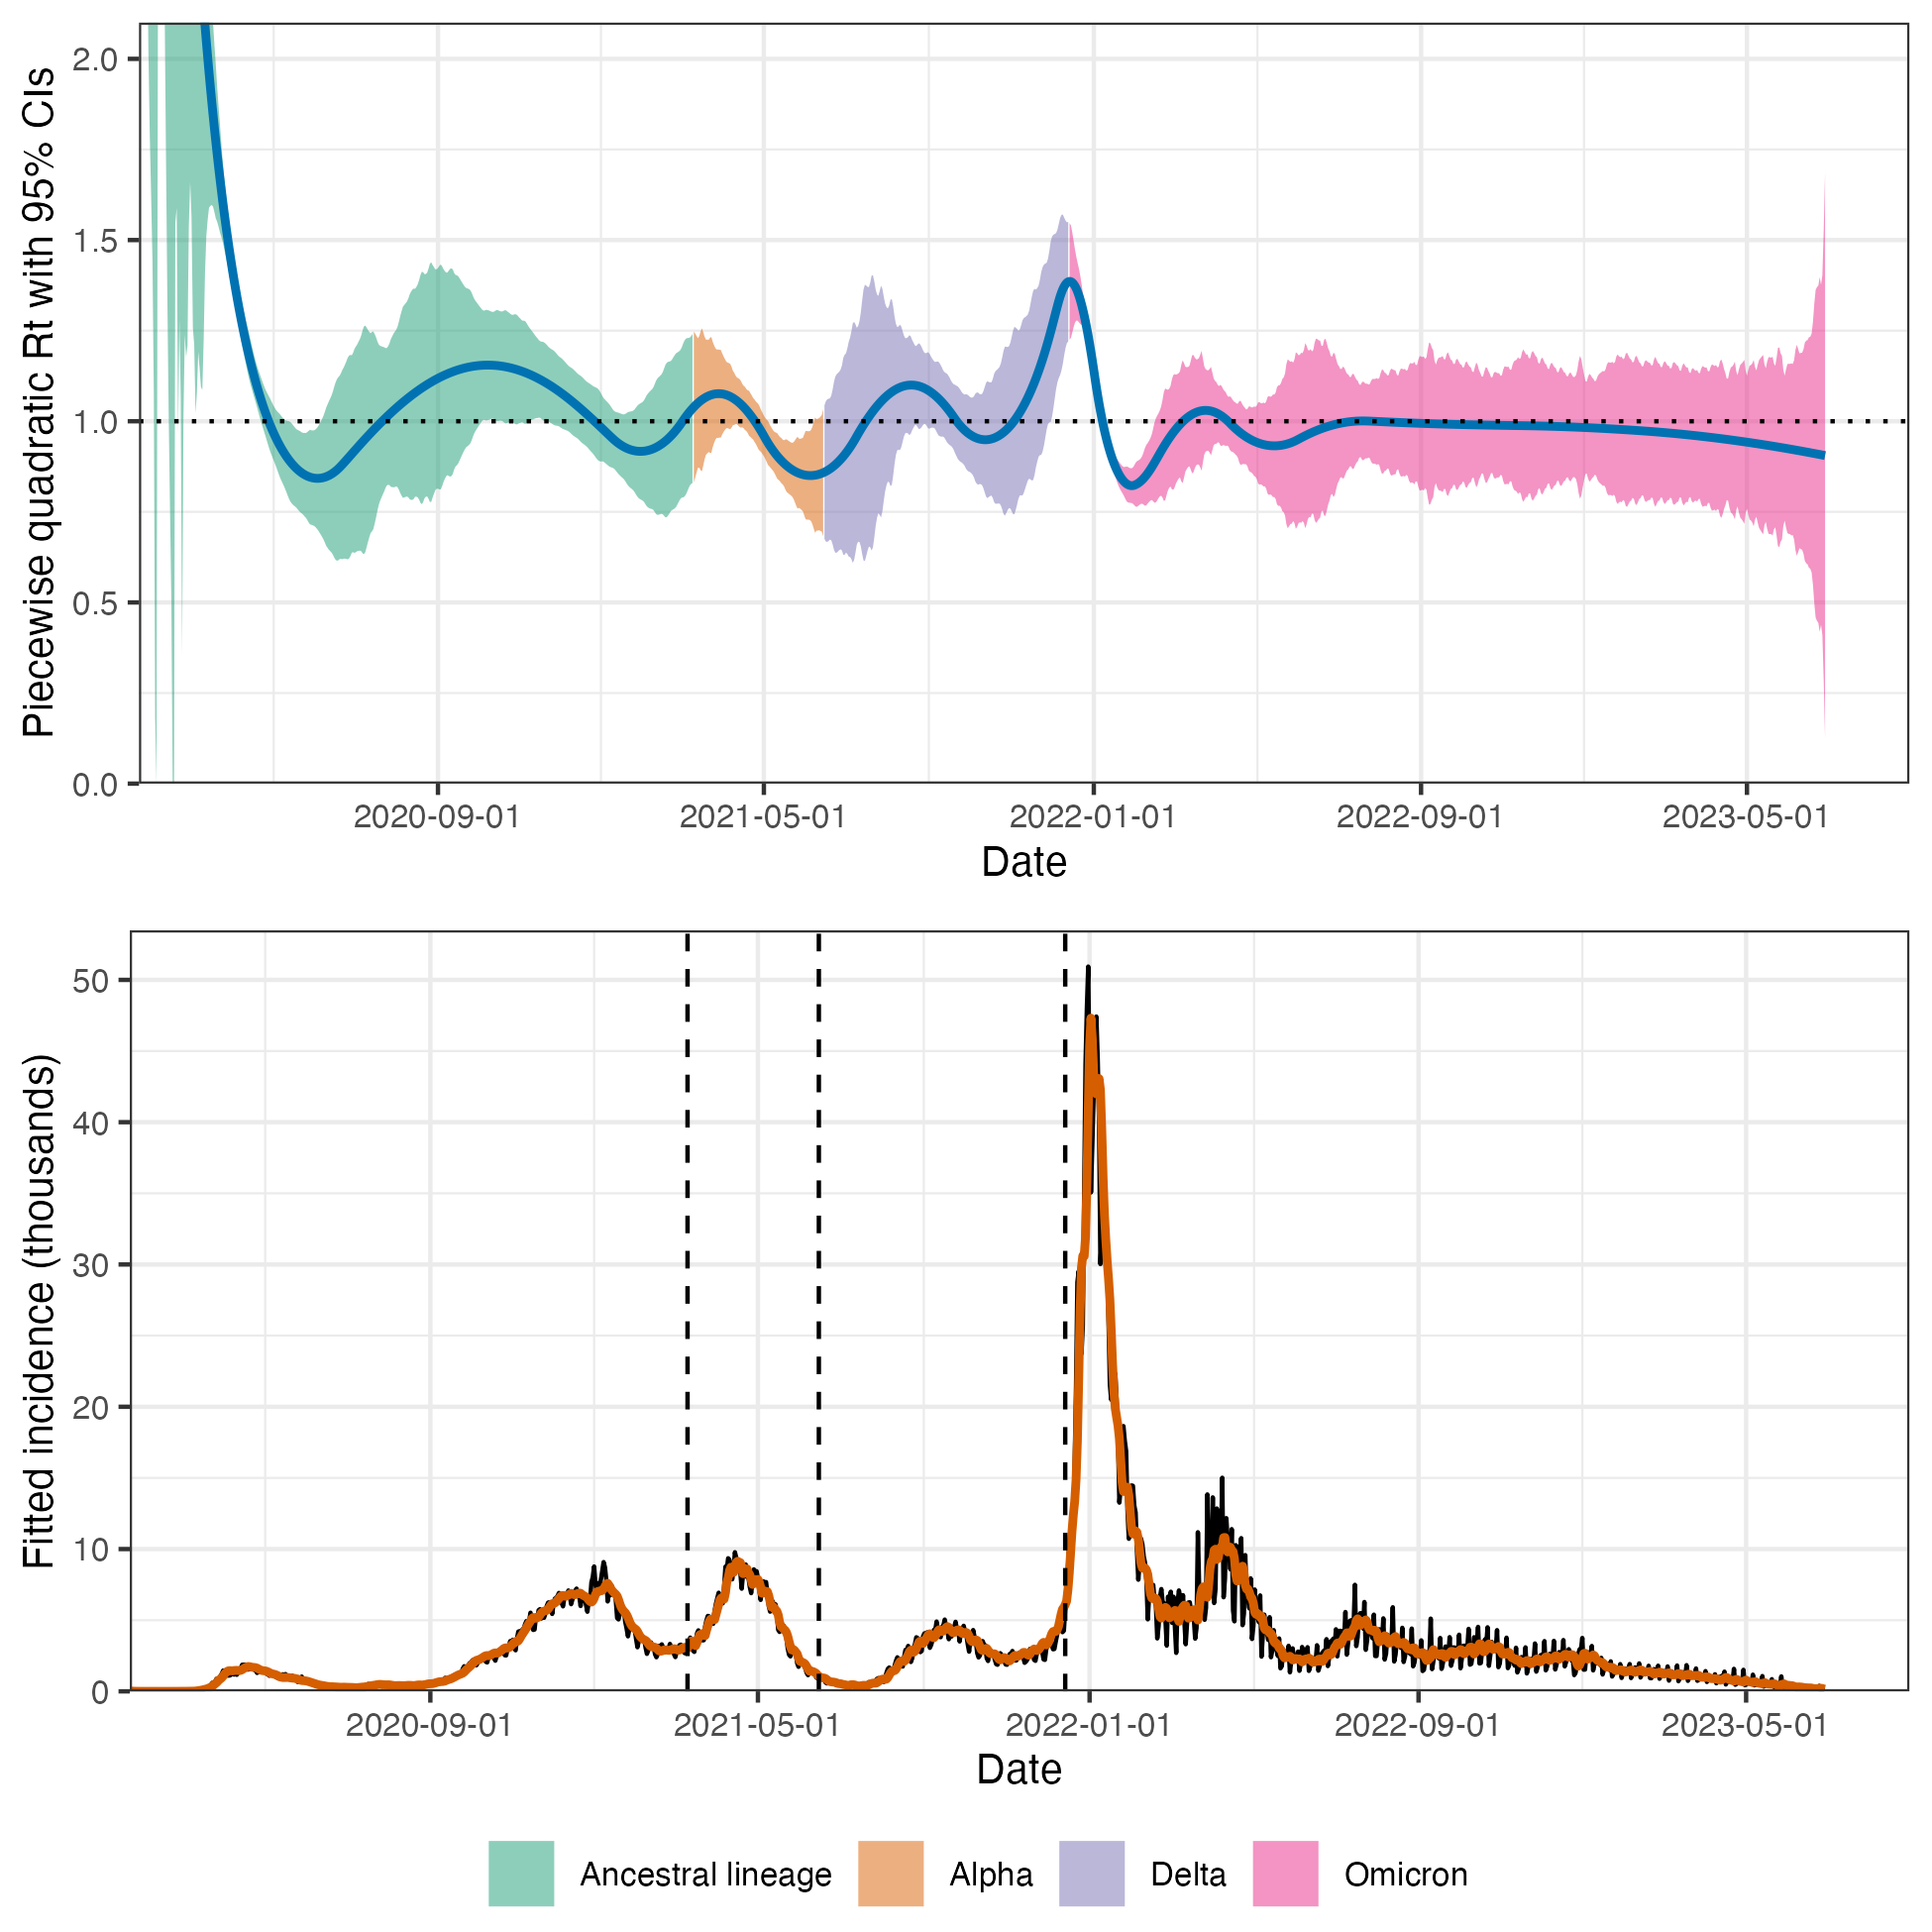
\includegraphics[width=1.0\textwidth]{fig/Fig1.png}
  \caption{{\bf A demonstration of instantaneous reproduction number estimation by
  \RtEstim\ and the corresponding predicted incident cases.} The example is the Covid-19
  epidemic in Canada during the period from January 23, 2020 to June 28, 2023.
  In the top panel, the blue curve is the estimated piecewise quadratic
  $\calR_t$ and the colorful ribbon is the corresponding 95\% confidence band.
  The colors represent the variants whose serial interval distributions are used
  to estimate $\calR_t$. The dominant circulating variants are based on a
  multinomial logistic regression model with variant probabilities from
  \cite{duotang_2023}. The time-varying serial interval distributions are 
  based on results from \cite{xu2023assessing}. 
  In the bottom panel, the black curve is the observed Covid-19
  daily confirmed cases, and the orange curve on top of it is the predicted
  incident cases corresponding to the estimated $\calR_t$. The three vertical
  dashed lines represent the beginning of a new dominant variant.}
  \label{fig:intro-fig}
\end{figure}

While our approach is straightforward and requires little domain knowledge for
implementation, we also implement a number of refinements:
\begin{itemize}
  \item the algorithm solves over a range of tuning parameters simultaneously,
  using warm starts to speed up subsequent solutions;
  \item cross-validation is built in (and used in all analyses below) to
  automatically select tuning parameters;
  \item parametric (gamma), non-parametric (any discretized delay), and
  time-varying delay distributions are allowed;
  \item irregularly spaced incidence data are easily accommodated;
  \item approximate confidence intervals for $\calR_t$ and the observed
  incidence are available;
  \item the estimated $\log\calR_t$ can be mathematically described as an
  element of a well-known function space depending on user choice \cite{tibshirani2022divided}.
\end{itemize}
We use a proximal Newton method to solve the convex optimization problem along
with warm starts to produce estimates efficiently, typically in a matter of
seconds, even for long sequences of data. In a number of simulation experiments,
we show empirically that our approach is more accurate than existing methods at
estimating the true instantaneous reproduction numbers and robust to some
degrees of misspecification of incidence distribution, serial interval
distribution, and the order of graphical curvature. 


The manuscript proceeds as follows. We first introduce the methodology of
\RtEstim\ including the renewal equation and the development of Poisson trend
filtering estimator. We explain how this method could be interpreted from the
Bayesian perspective, connecting it to previous work in this context. We provide
illustrative experiments comparing our estimator to other Bayesian alternatives.
We then apply our \RtEstim\ on the Covid-19 pandemic in Canada and the 1918
influenza pandemic in the United States. Finally, we conclude with a discussion
of the advantages and limitations of our approach and describe some practical
considerations for instantaneous reproduction number estimation.


\section{Methods}

\subsection{Renewal model for incidence data} 

The instantaneous reproduction number $\calR(t)$ is defined to be the expected
number of secondary infections at time $t$ produced by a primary infection
sometime in the past. To make this precise, denote the number of new infections
at time $t$ as $y(t)$. Then the total primary infectiousness can be written as
$\eta(t) := \int_0^{\infty} p(t,i) y(t-i) \diff i$, where $p(t,i)$ is the
probability that a new secondary infection at time $t$ is the result of a
primary infection that occurred $i$ time units in the past. The instantaneous
reproduction number is then given as the value that equates
\begin{equation} \label{eq:pre-renew-equation}
  \bbE[y(t) \mid y(j),\ j<t]=\calR(t)\eta(t)=\calR(t)\int_0^\infty p(t,i)y(t-i)\diff i,
\end{equation}
otherwise known as the renewal equation. The period between primary and
secondary infections is exactly the generation time of the disease, but given
real data, observed at discrete times (say, daily), this delay distribution must
be discretized into contiguous time intervals, say, $(0,1], (1,2], \ldots$,
resulting in the sequence $\{p_{t,i}\}_{i=0}^\infty$ corresponding to
observations $y_t$ for each $t$ and yields the discretized version of
\eqref{eq:pre-renew-equation},
\begin{equation} \label{eq:renew-equation}
  \bbE[y_t \mid y_1,\ldots,y_{t-1}]=\calR_t\eta_t=\calR_t\sum_{i = 1}^\infty p_{t,i} y_{t-i}.
\end{equation}
Many approaches to estimating $\calR_t$ rely on \eqref{eq:renew-equation} as
motivation for their procedures, among them, \EpiEstim\ \cite{cori2013new} 
and \texttt{EpiFilter} \cite{parag2021improved}. 


In most cases, it is safe to assume that infectiousness disappears beyond $\tau$
timepoints ($p(t,i) = 0$ for $i > \tau$), resulting in the truncated integral of
the generation interval distribution $\int_0^\tau p(t,i)\diff i = 1$ for each
$t$. Generation time, however, is usually unobservable and tricky to estimate,
so common practice is to approximate it by the serial interval: the period
between the symptom onsets of primary and secondary infections. If the
infectiousness profile after symptom onset is independent of the incubation
period (the period from the time of infection to the time of symptom onset),
then this approximation is justifiable: the serial interval distribution and the
generation interval distribution share the same mean. However, other properties
may not be similarly shared, and, in general, the generation interval
distribution is a convolution of the serial interval distribution with the
distribution of the difference between independent draws from the delay
distribution from infection to symptom onset. See, for example,
\cite{gostic2020practical} for a fuller discussion of the dangers of this
approximation. Nonetheless, treating these as interchangeable is common
\cite{cori2013new,park2021forward}, and doing otherwise is beyond the scope of
this work. We will allow the delay distribution to be either constant over time---the probability $p(i)$ depends only on the gap between primary and
secondary infections and not on the time $t$ when the secondary infection
occurs---or to be time-varying: $p(t,i)$ also depends on the time of the
secondary infection. For our methods, we assume that the serial interval can be
accurately estimated from auxiliary data (say by contact tracing, or previous
epidemics) and we take it as fixed, as is common in existing studies,
\cite{cori2013new,abry2020spatial,pascal2022nonsmooth}.


The renewal equation in \eqref{eq:renew-equation} relates observable data
streams (incident cases) occurring at different timepoints to the instantaneous
reproduction number given the serial interval. The fact that it depends only on
the observed incident counts makes it reasonable to estimate $\calR_t$. However,
data collection idiosyncrasies can obscure this relationship. Diagnostic testing
targets symptomatic individuals, omitting asymptomatic primary infections which
can lead to future secondary infections. Testing practices, availability, and
uptake can vary across space and time \cite{pitzer2021impact,
hitchings2021usefulness}. Finally, incident cases as reported to public health
are subject to delays due to laboratory confirmation, test turnaround times, and
eventual submission to public health \cite{pellis2021challenges}. For these
reasons, reported cases are lagging indicators of the course of the pandemic.
Furthermore, they do not represent the actual number of new infections that
occur on a given day, as indicated by exposure to the pathogen. The assumptions
described above (homogeneous mixing, similar susceptibility and social
behaviours, etc.) are therefore consequential. That said,
\eqref{eq:renew-equation} also provides some comfort about deviations from these
assumptions. Under certain conditions, failing to account for the reporting
behaviours will minimally impact the accuracy of any $\mathcal{R}_t$ estimator
that is based on \eqref{eq:renew-equation}. We discuss three types of deviation
here. First, if $y_t$ is scaled by a constant $a$ describing the reporting
ratio, then, because it appears on both sides of \eqref{eq:renew-equation},
$\calR_t$ will be unchanged. Second, if such a scaling $a_t$ varies in time, as
long as it varies slowly relative to $p_i$ ---that is, if $a_t / \sum_{i = 1}^t
a_i p_i \approx 1$---then $\calR_t$ can still be estimated well from reported
incidence data. Finally, if a sudden change in reporting ratio occurs at time
$t_1$, it would only result in large errors in $\calR_t$ at times near $t_1$
(where the size of this neighbourhood is determined indirectly by the effective
support of $\{p_{t_1,i}\}$). On the other hand, time-varying reporting delays
would be much more detrimental \cite{EALES2024100742,park2024estimating}.


\subsection{Poisson trend filtering estimator} 

We use the daily confirmed incident cases $y_t$ on day $t$ to estimate the
observed infectious cases under the model that $y_t$, given previous incident
cases $y_{t-1},\ldots,y_1$ and a constant serial interval distribution, follows a
Poisson distribution with mean $\Lambda_t$. That is, 
\begin{equation}
  y_t \mid y_1,\ldots,y_{t-1} \sim \mathrm{Poisson}(\Lambda_t), \textrm{ where } 
  \Lambda_t =  \calR_t\sum_{i=1}^{t-1}p_i y_{t-i} = \calR_t\eta_t.
\end{equation} 
We will write $p_i$ as constant in time for simplicity, although this is not
required. Given a history of $n$ confirmed incident counts $\bfy =
{(y_1,\ldots,y_n)}^\top$,
our goal is to estimate $\calR_t$ for each $t=1,\ldots,n$. A natural approach is to maximize the
likelihood, producing the maximum likelihood estimator (MLE):
\begin{equation} \label{eq:mle}
  \begin{split}
    \widehat{\calR} &= \Argmax{\calR \in \bbR_+^n} \bbP(\calR \mid \bfy,\ \bfp)
    = \Argmax{\calR \in \bbR^n_+} \prod_{t = 1,\dots,n} 
    \frac{\lr{\calR_t \eta_t}^{y_t} \exp\{- \calR_t \eta_t\}  }{y_t!}\\
    &= \Argmin{\calR\in\bbR^n_+} \sum_{t = 1}^n \calR_t\eta_t - 
    y_t\log(\calR_t\eta_t).
  \end{split}
\end{equation}
This optimization problem, however, is easily seen to yield a one-to-one
correspondence between the observation and the estimated instantaneous reproduction
number, i.e.,
$\widehat{\calR}_t = y_t / \eta_t$, so that the estimated sequence
$\widehat{\calR}$ will have no significant smoothness.


The MLE is an unbiased estimator of the true parameter $\calR_t$, but
unfortunately has high variance: changes in $y_t$ result in proportional changes
in $\widehat\calR_t$. To avoid this behaviour, and to match the intuition that
$\calR_t \approx \calR_{t-1}$, we advocate enforcing smoothness of the
instantaneous reproduction numbers. This constraint will decrease the estimation
variance, and hopefully lead to more accurate estimation of $\calR$, as long as
the smoothness assumption is reasonable. Smoothness assumptions are common (see
e.g., \cite{gostic2020practical,parag2021improved}), but the type of smoothness
assumption is critical. Cori et al.\cite{cori2013new} imposes smoothness
indirectly by estimating $\calR_t$ with moving windows of past observations. The
Kalman filter procedure of \cite{parag2021improved} would enforce
$\ell_2$-smoothness ($\int_0^n {(\widehat{\calR}''(t))}^{2}\diff t < C$ for some
constant $C$), although the computational implementation results in
$\widehat{\calR}$ taking values over a discrete grid. Pascal et
al.\cite{pascal2022nonsmooth} produces piecewise linear $\widehat{\calR}_t$,
which turns out to be closely related to a special case of our methodology.
Smoother estimated curves will provide high-level information about the entire
epidemic, obscuring small local changes in $\calR(t)$, but may also remove the
ability to detect large sudden changes, such as those resulting from lockdowns
or other major containment policies. 

To enforce smoothness of $\hat\calR_t$, we add a trend filtering penalty 
\cite{kim2009ell_1, tibshirani2014adaptive, tibshirani2022divided, sadhanala2024exponential} 
to \eqref{eq:rt-ptf} . Because $\calR_t > 0$,
we explicitly penalize the divided differences (discrete derivatives) of
neighbouring values of $\log(\calR_t)$. 
Let $\theta := \log(\calR) \in \bbR^n$, so that $\Lambda_t =
\eta_t \exp(\theta_t)$, and $\log(\eta_t \calR_t) = \log(\eta_t) +
\theta_t$. For evenly spaced incidence data, we
write our estimator as the solution to the optimization problem
\begin{equation} 
  \label{eq:rt-ptf}
  \widehat{\calR} = \exp(\widehat{\theta}) \quad\textrm{where}\quad \widehat{\theta} 
  = \Argmin{\theta\in\bbR^n} \eta^\top \exp(\theta) - \bfy^\top \theta + \lambda 
  \snorm{D^{(k+1)} \theta}_1,
\end{equation}
where $\exp(\cdot)$ applies elementwise and $\snorm{\boldsymbol{a}}_1 :=
\sum_{i=1}^n |a_i|$ is the $\ell_1$ norm. Here, $D^{(k+1)} \in
\bbZ^{(n-k-1)\times n}$ is the $(k+1)\th$ order divided difference matrix for
any $k \in \{0,\ldots,n-1\}$ with the convention that $D^{(0)} = \mathbf{0}_{n
\times n}$. The divided difference matrix for $k=0$, $D^{(1)} \in \{-1,0,1\}^{(n-1)\times n}$, is a sparse matrix with diagonal band of
the form:
\begin{equation} 
  \label{eq:d1mat}
  D^{(1)} = 
  \begin{pmatrix} 
    -1 & 1 &  & & \\ 
    & -1 & 1 & & \\ 
    & & \ddots & \ddots & \\
    & & & -1 & 1 
  \end{pmatrix}.
\end{equation}
For $k\geq 1$, $D^{(k+1)}$ can be defined recursively as $D^{(k+1)} := D^{(1)}
D^{(k)}$, where $D^{(1)} \in \{-1,0,1\}^{(n-k-1)\times (n-k)}$ has the form
\eqref{eq:d1mat} but with modified dimensions.

The tuning parameter (hyperparameter) $\lambda$ balances data
fidelity with desired smoothness. When $\lambda=0$, the problem in
\eqref{eq:rt-ptf} reduces to the MLE in \eqref{eq:mle}. Larger tuning parameters
privilege the regularization term and yield smoother estimates. Finally, there
exists $\lambda_{\textrm{max}}$ such that any $\lambda \geq
\lambda_{\textrm{max}}$ will result in $D^{(k+1)} \widehat {\theta} = 0$ and
$\widehat{\theta}$ will be the Kullback-Leibler projection of $\bfy$ onto the
null space of $D^{(k+1)}$ (see \autoref{sec:candidate-set} for more details).

The solution to \eqref{eq:rt-ptf} will result in piecewise
polynomials, specifically called discrete splines. For example, $0\th$-degree
discrete splines are piecewise constant, \first-degree curves are piecewise
linear, and \second-degree curves are piecewise quadratic. For $k\geq 1$,
$k\th$-degree discrete splines are continuous and have continuous discrete
differences up to degree $k-1$ at the knots (i.e., changing points between segments). This penalty results in more
flexibility compared to the homogeneous smoothness that is created by the
squared $\ell_2$ norm. Using different orders of the divided differences results in
estimated instantaneous reproduction numbers with different smoothness properties. 



For unevenly spaced data, the spacing between neighbouring parameters
varies with the time between observations, and thus, the divided differences
must be adjusted by the times that the observations occur. Given observation
times $\bfx = {(x_1,\dots,x_n)}^\top$, for $k \geq 1$, define a $k\th$-order
diagonal matrix 
\begin{equation}
  X^{(k)} = \diag \lr{\frac{k}{x_{k+1} - x_1},\ \frac{k}{x_{k+2} - x_2},\ 
  \cdots,\ \frac{k}{x_n - x_{n-k}} }.
\end{equation}
Letting $D^{(\bfx,1)} := D^{(1)}$,
then for $k\geq 1$, the $(k+1)\th$-order divided difference matrix for unevenly
spaced data can be created recursively by
$D^{(\bfx, k+1)} := D^{(1)} X^{(k)} D^{(\bfx,k)}.$ No adjustment is required
for $k=0$. 


Due to the penalty structure, this estimator is locally adaptive, meaning that
it can potentially capture local changes such as the initiation of control
measures, becoming more wiggly in regions that require it. In contrast, Abry et
al.\ and Pascal et al.\ considered only the \second-order ($k = 1$) divided
difference of $\calR_t$ rather than its logarithm
\cite{abry2020spatial,pascal2022nonsmooth}. In comparison to their work, our
estimator (i) allows for arbitrary degrees of temporal smoothness and (ii)
avoids the potential numerical issues of penalizing/estimating positive real
values. Nonetheless, as we will describe below, our procedure is computationally
efficient for estimation over an entire sequence of hyperparameters $\lambda$
and provides methods for choosing how smooth the final estimate should be.


\subsection{Solving over a sequence of tuning parameters}
\label{sec:candidate-set}

We can solve the Poisson trend filtering estimator over an arbitrary sequence of 
$\lambda$ that produces different levels of smoothness in the estimated curves. 
We consider a candidate set of M $\lambda$-values, $\boldsymbol{\lambda} = \{\lambda_m\}_{m=1}^M$,
that is strictly decreasing.


Let $D := D^{(k+1)}$ for simplicity in the remainder of this section. As
$\lambda \to\infty$, the penalty term $\lambda \snorm{D\theta}_1$ dominates the
Poisson loss, so that minimizing \eqref{eq:rt-ptf} is asymptotically equivalent
to minimizing the penalty term, which results in $\snorm{D\theta}_1 = 0$. In
this case, the divided differences of $\theta$ with order $k+1$ is always $0$,
and thus, $\theta$ must lie in the null space of $D$, that is,
$\theta\in\mathcal{N}(D)$. The same happens for any $\lambda$ beyond this
threshold, so define $\lambda_{\textrm{max}}$ to be the smallest $\lambda$ that
produces $\theta\in\mathcal{N}(D)$. It turns out that this value can be written
explicitly as $\lambda_{\textrm{max}} = \snorm{\lr{D^{\dagger}}^{\top} \lr{\eta
- y}}_{\infty},$ where $D^{\dagger}$ is the (left) generalized inverse of $D$
satisfying $D^{\dagger} D = I$ and $\snorm{a}_{\infty} :=
\mathrm{max}_{i}|a_i|$ is the infinity norm. Explicitly, for any $\lambda \geq
\lambda_{\max}$, the solution to \eqref{eq:rt-ptf} will be identical to the
solution with $\lambda_{\max}$. Therefore, we use
$\lambda_1 = \lambda_{\max}$ and choose the minimum $\lambda_M$ to
be $r\lambda_{\max}$ for some $r \in (0,1)$ (typically $r=10^{-4}$). Given any
$M\geq 3$, we generate a sequence of $\lambda$ values to be equally spaced on
the log-scale between $\lambda_1$ and $\lambda_M$. 

To compute the sequence of solutions efficiently, the model is estimated
sequentially by visiting each $\lambda_m$ in order, from largest to smallest. The
estimates produced for a larger $\lambda$ are used as the initial values (warm
starts) for the next smaller $\lambda$. By solving through the entire sequence
of tuning parameters, we improve computational efficiency and also enable one to
trade between bias and variance, resulting in improved accuracy relative to
procedures using a single fixed tuning parameter.


\subsection{Choosing a final $\lambda$}
\label{sec:cv}

We estimate model accuracy over the candidate set through $V$-fold cross
validation (CV) to choose the best tuning parameter. Specifically, we divide
$\bfy$ (except the first and last observations) roughly evenly and randomly into
$V$ folds, estimate $\calR_t$ for all $\boldsymbol{\lambda}$ leaving one fold
out, and then predict the held-out observations. Alternativly, one could use
regular splitting, assigning every $v\th$ observation into the same fold. Note
that our approach is most closely related to non-parametric regression rather
than time series forecasting. That said, under some conditions, one can
guarantee that $V$-fold remains valid for risk estimation in time series. The
sufficient conditions are quite strong, but the guarantees are also stronger
than would be required for model selection consistency \cite{BERGMEIR201870}. 


Model accuracy can be measured by multiple metrics such as mean squared error
$\mathrm{MSE}(\widehat{y},\ y) = n^{-1}\snorm{\widehat{y} - y}_2^2$ or mean
absolute error $\mathrm{MAE}(\widehat{y},\ y) = n^{-1}\snorm{\widehat{y} -
y}_1$, but we prefer to use the (average) deviance, to mimic the likelihood in
\eqref{eq:mle}: $D\lr{y,\ \hat{y}} = n^{-1}\sum_{i=1}^n 2\lr{y_i \log(y_i) -
y_i\log(\hat{y}_i) - y_i + \hat{y}_i},$ with the convention that $0\log(0) = 0$.
Note that for any $V$ and any $M$, we will end up estimating the model $(V+1)M$
times rather than once.


\subsection{Approximate confidence bands} 
\label{sec:conf-band} 

We also provide empirical confidence bands of the estimators with  
approximate coverage. Consider the related estimator $\widetilde{\calR}_t$
defined as
\begin{equation}
  \widetilde{\calR} = \exp(\widetilde{\theta}) \quad\textrm{where}\quad
  \widetilde{\theta} = \Argmin{\theta\in\bbR^n} \eta^\top \exp(\theta) - \bfy^\top
  \theta + \lambda \snorm{D \theta}_2^2.
\end{equation}
Letting $\widetilde{\bfy} = \eta \circ \widetilde\calR$ (where $\circ$ denotes the
elementwise product), it can be shown
(for example, Theorem 2 in \cite{vaiter2017degrees}) that an estimator for
$\Var(\widetilde{\bfy})$ is given by $\big(\mathrm{diag}(\widetilde{\bfy}^{-2})
+ \lambda D^{\top} D\big)^{\dagger}.$ Finally, an application of the delta
method shows that $\Var(\widetilde{\bfy}_t) / \eta_t^2$ is an estimator for
$\Var(\widetilde{\calR}_t)$ for each $t = 1, \ldots, n$. We therefore use
${\big(\mathrm{diag}(\widehat{\bfy}^{-2}) + \lambda D^{\top} D\big)}^{\dagger}_t
/ \eta_t^2$ as an estimator for $\Var(\widehat{\calR}_t)$. An approximate
$(1-\alpha)\%$ confidence interval then can be written as $\widehat{\calR}_t\pm
s_t \times T_{\alpha/2,n-\textrm{df}}$, where $s_t$ is the square-root of
$\Var(\widehat{\calR}_t)$ for each $t = 1, \cdots, n$ and $\textrm{df}$ is the
number of changepoints in $\widehat{\theta}$ plus $k+1$
\cite{tibshirani2014adaptive}. An approximate confidence interval of
$\hat{\bfy}$ can be computed similarly. 


\subsection{Bayesian perspective}

Unlike many other methods for $\calR_t$ estimation, our approach is frequentist
rather than Bayesian. Nonetheless, it has a corresponding Bayesian
interpretation: as a state-space model with Poisson observational noise,
autoregressive transition equation of degree $k\geq 0$, e.g., $\theta_{t+1} =
2\theta_t - \theta_{t-1} + \varepsilon_{t+1}$ for $k=1$, and Laplace transition
noise $\varepsilon_{t+1}\sim \mathrm{Laplace}(0,\ 1/\lambda)$. Compared to
\texttt{EpiFilter} \cite{parag2021improved},
 we share the same observational assumptions, but our approach has a
different transition noise. \texttt{EpiFilter} estimates the posterior
distribution of
$\calR_t$, and thus it can provide credible interval estimates as well. Our
approach produces the maximum \emph{a posteriori} estimate via an efficient
convex optimization, obviating the need for MCMC sampling. But the associated
confidence bands are created differently.


\section{Results}

Implementation of our approach is provided in the \R\ package
\href{https://dajmcdon.github.io/rtestim/}{\texttt{rtestim}}. All computational
experiments are conducted on the Cedar cluster provided by the Digital Research
Alliance of Canada with \texttt{R 4.3.1}. The \R\ packages used for simulation
and real-data application are \texttt{EpiEstim 2.2-4} \cite{Cori2022},
\texttt{EpiLPS 1.2.0} \cite{Gressani2021}, and \texttt{rtestim 0.0.4}. The \R\
scripts for \EpiFilter\ are used \cite{kpzoo2020}.

\subsection{Synthetic experiments}

\subsubsection{Design for the synthetic data}

We simulate four scenarios of the instantaneous reproduction number, intended to
mimic different epidemics. The first two scenarios are rapidly controlled by
intervention, where the $\calR(t)$ consists of one discontinuity and two
segments. Scenario 1 has constant $\calR(t)$ before and after an intervention,
while Scenario 2 grows exponentially, then decays. The other two scenarios are
more complicated, where more waves are involved. Scenario 3 has four linear
segments with three discontinuities, which reflect the effect of an
intervention, resurgence to rapid transmission, and finally suppression of the
epidemic. Scenario 4 involves sinusoidal waves throughout the epidemic. The
first three scenarios and the last scenario are motivated by
\cite{parag2021improved} and \cite{gressani2022epilps} respectively. We name the
four scenarios as (1) piecewise constant, (2) piecewise
exponential, (3) piecewise linear, and (4) periodic.

In all cases, the times of observation are regular, and epidemics are of length
$n=300$. Specifically, in Scenario 1, $\calR_t = 2$ for $t\leq 120$ and 0.8 for $t>120$. In
Scenario 2, $\calR_t$ increases and decreases exponentially with rates $0.01$
for $t\leq 100$ and 0.005 for $t>100$. In Scenario 3, $\calR_t$ is piecewise linear
with four discontinuous segments, 
\begin{equation}
  \begin{split}
    \calR(t) =& \lr{2.5 - \frac{0.5}{74}\lr{t-1}} \boldsymbol{1}_{[1,76)}(t)
     + \lr{0.8 - \frac{0.2}{74}\lr{t-76}} \boldsymbol{1}_{[76,151)}(t) \\
    & + \lr{1.7 + \frac{0.3}{74}\lr{t-151}} \boldsymbol{1}_{[151,226)}(t)
       + \lr{0.9 - \frac{0.4}{74}\lr{t-226}} \boldsymbol{1}_{[226,300]}(t),
  \end{split}
\end{equation}
where $\boldsymbol{1}_{A}(t) = 1$, if $t\in A$, and $\boldsymbol{1}_{A}(t)=0$ otherwise. 
In Scenario 4, $\calR_t$ is realization of the 
continuous, periodic curve generated by the function 
\begin{equation}
  \calR(t) = 0.2 \big(\lr{\sin(\pi t/12) + 1} + \lr{2 \sin\lr{5 \pi t / 12} + 2} 
  + \lr{3 \sin(5\pi t / 6) + 3}\big),
\end{equation} 
evaluated at equally spaced points $t\in [0,10]$. These $\calR_t$ scenarios are
illustrated in \autoref{fig:samples}. We compute the expected incidence
$\Lambda_t$ using the renewal equation, and generate the incident infections
from the Poisson distribution with mean $\bbE[y_t \mid y_s,\ s<t] = \Lambda_t$.
To verify the performance of our model under violations of the model's
distributional assumptions, we also generate incident cases using the negative
binomial distribution with dispersion parameter $\rho = 5$. Here, the negative
binomial is parameterized such that the mean is
$\bbE[y_t\mid y_s,\ s<t] = \Lambda_t$ and the variance is $\textrm{Var}[y_t \mid
y_s,\ s<t] = \Lambda_t(1 +
\Lambda_t / \rho)$ (following, for example, \cite{gressani2022epilps}). Because
$(1 + \Lambda_t / \rho)> 1$ for  $0\leq\rho <\infty$, this parameterization results
in overdispersion relative to the Poisson distribution, with smaller values of
$\rho$ leading to greater overdispersion. For context on the observed dispersion
of these synthetic experiments, Figure A.2.1 in \nameref{S1_supp} displays the
ratio of the time-varying standard deviation to the mean. 

We use serial interval (SI) distributions of measles (with mean $14.9$ and
standard deviation $3.9$) in Hagelloch, Germany in 1861
\cite{groendyke2011bayesian} and SARS (with mean $8.4$ and standard deviation
$3.8$) in Hong Kong in 2003 \cite{lipsitch2003transmission}, inspired by
\cite{cori2013new}, to generate synthetic epidemics. We initialize all epidemics
with $y_1=2$ cases and generate for $t=2,\ldots,300$. The synthetic measles
epidemics have smaller incident cases in general, and the SARS epidemics have
larger incidence. Essentially, the smaller mean of the serial interval for SARS
with a similar standard deviation leads to shorter expected delays between
onsets of primary and secondary infections, resulting in faster growth of
incidence within the same period of time. We also consider shorter flu epidemics
with 50 timepoints with piecewise linear $\calR_t$ (Scenario 3) considering both
incidence distributional assumptions. The motivation is to compare our method
and other alternatives with EpiNow2 which takes much longer to compute for long
epidemics (nearly 2 hours to converge for a measles epidemic with 300
timepoints) than other methods. Besides using the correct SI distributions to
estimate $\calR_t$, we also consider the scenarios where the SI is misspecified.
More details on experimental settings and results for shorter epidemics and
misspecification of SI distributions are given in Sections A.2.1 and A.3 in the
supplementary document respectively. 

For each problem setting (including SI distribution, an $\calR_t$ scenario, and
an incidence distribution), we generate 50 random samples, resulting in $800$
total synthetic epidemics. Example realizations for measles and SARS with each
instantaneous reproduction number scenario is displayed in
\autoref{fig:samples}. 

\begin{figure}[!t]
  \centering
  %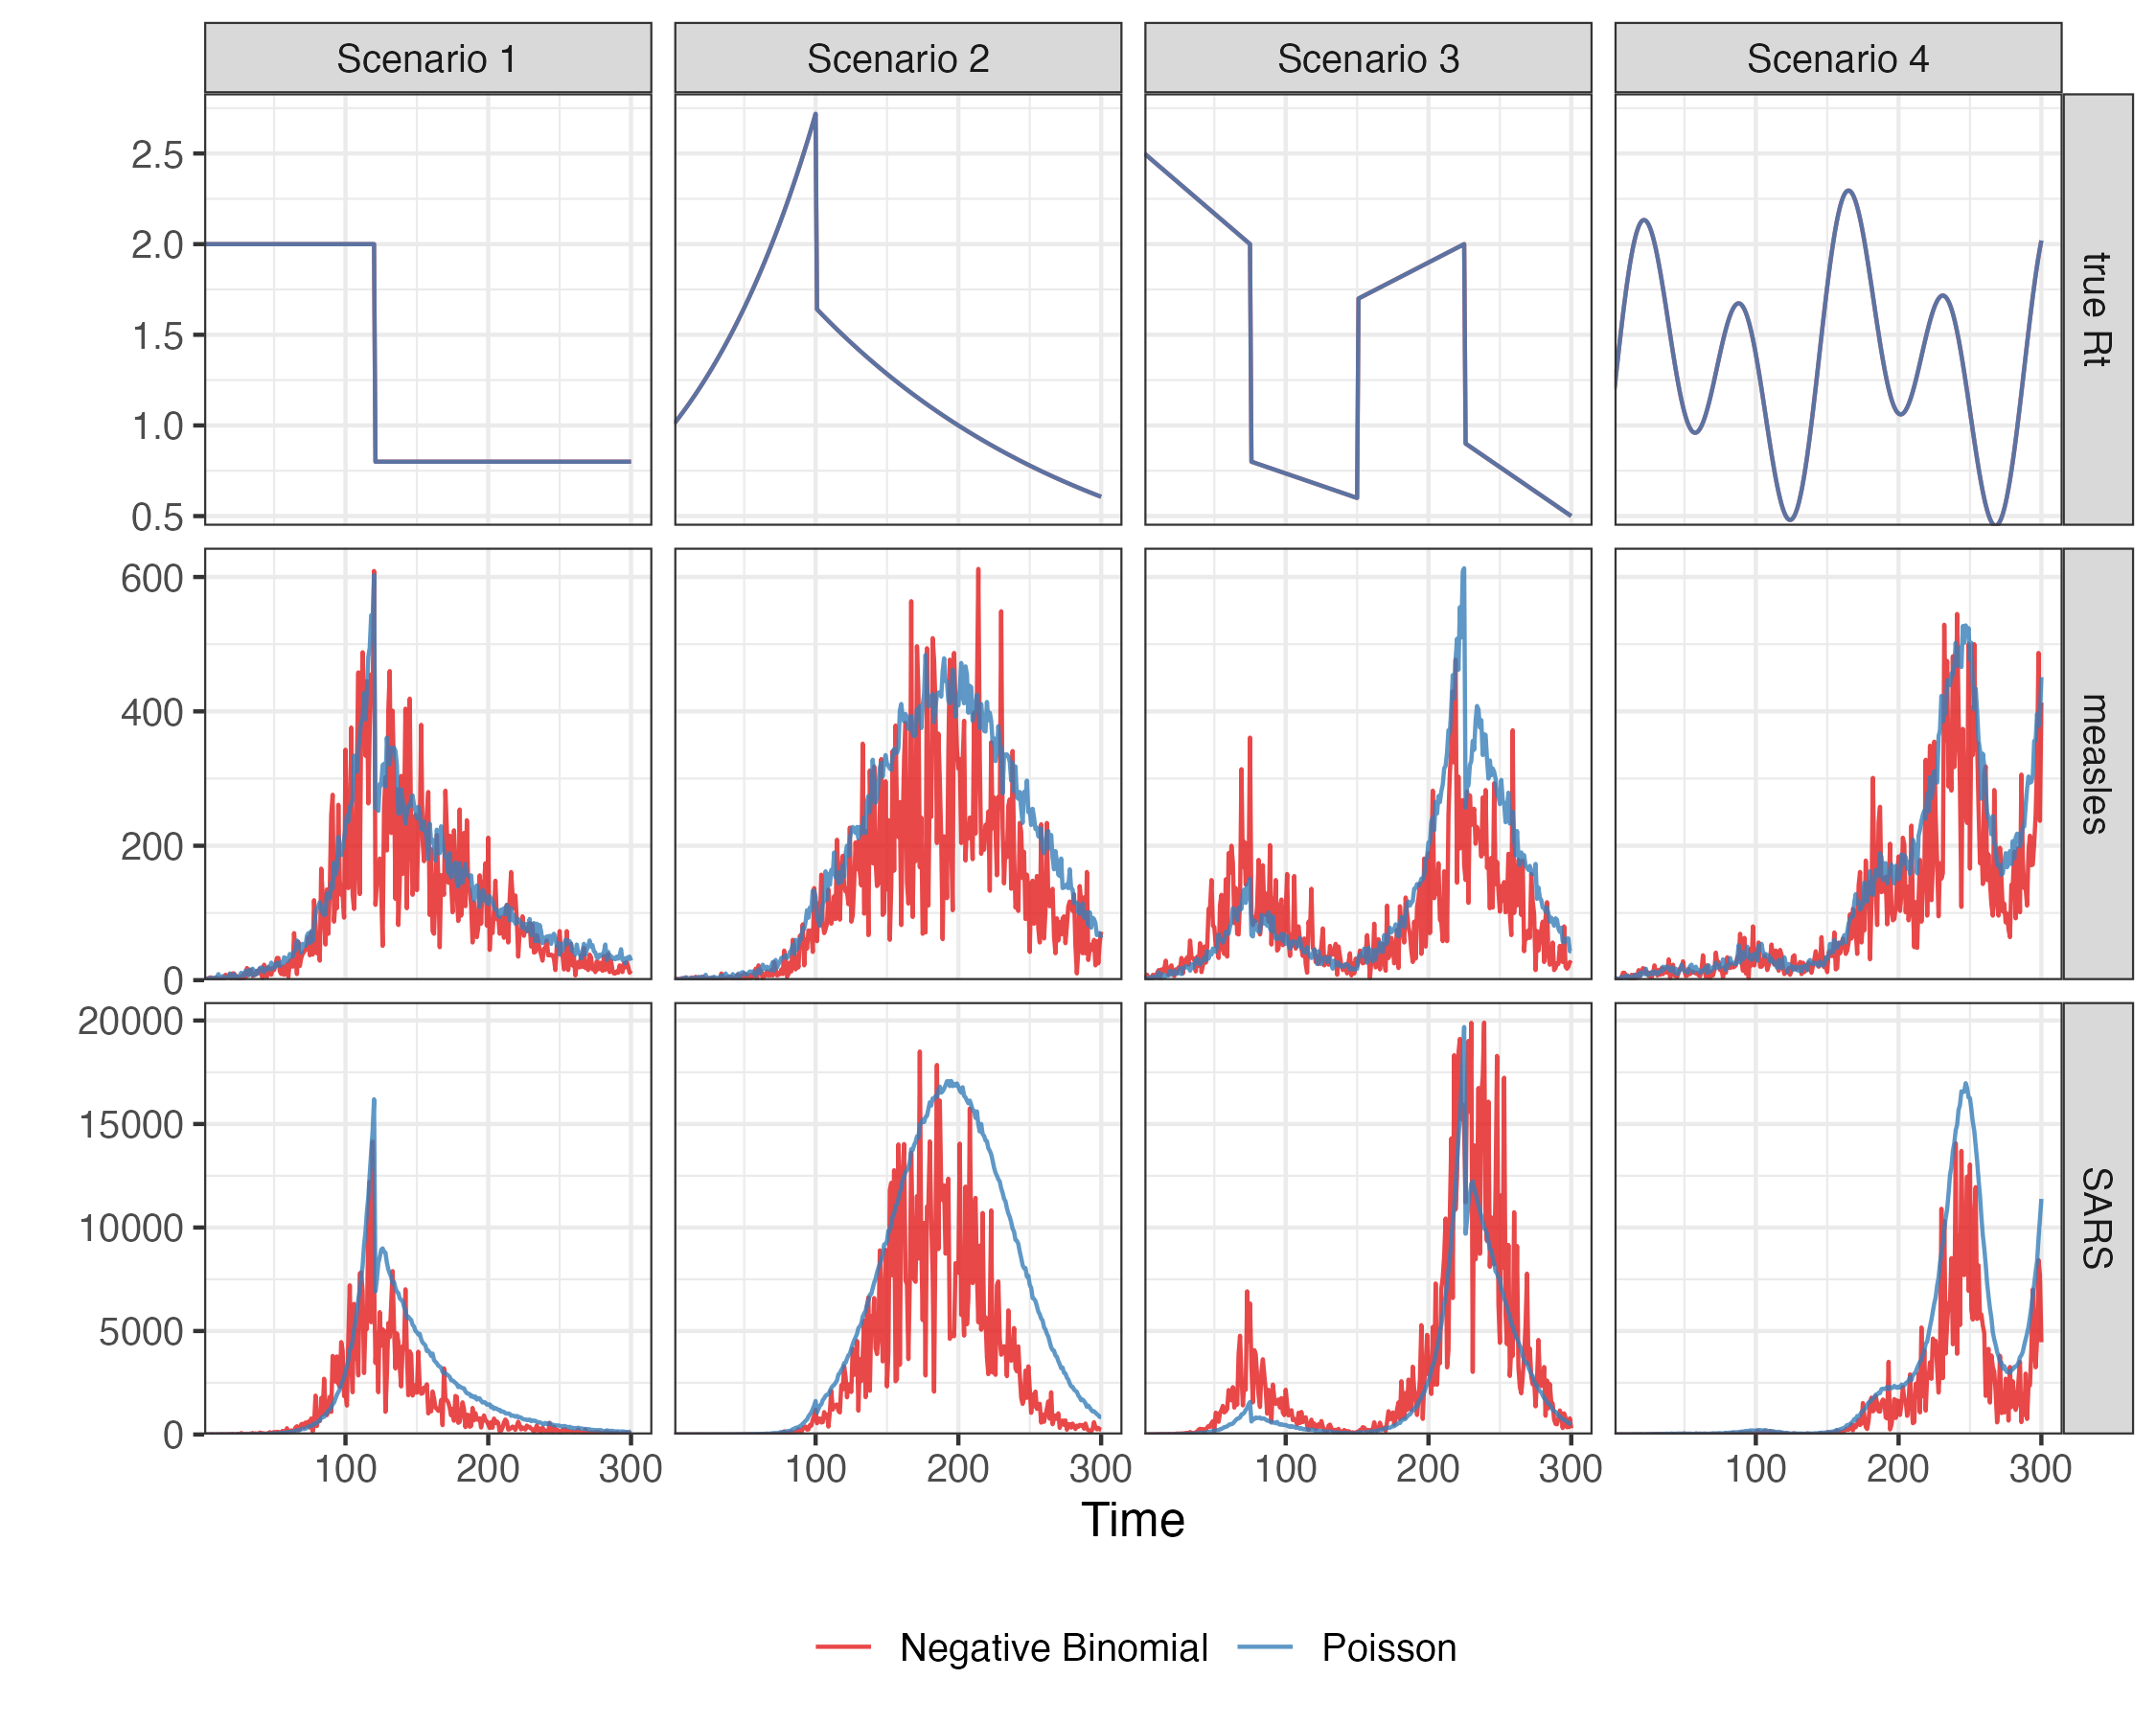
\includegraphics[width=1.0\linewidth]{fig/Fig2.png}
  \caption{{\bf This figure displays example realizations for each $\calR_t$ setting.}
  Top row: the instantaneous reproduction numbers. Middle row: synthetic measles
  incidence (Poisson in blue, negative binomial in red) incidence. Bottom row:
  synthetic SARS incidence. The 4 4 $\calR_t$ scenarios are shown in the
  columns.} 
  \label{fig:samples}
\end{figure}

\subsubsection{Algorithmic choices}

We compare \RtEstim\ to \EpiEstim, \EpiLPS, and \EpiFilter. \EpiEstim\ estimates
the posterior distribution of the instantaneous reproduction number given a
Gamma prior and Poisson distributed observations over a trailing window, under
the assumption that the instantaneous reproduction number is constant during
that window. A larger window averages out more fluctuations, leading to smoother
estimates, whereas a shorter window is more responsive to sudden spikes or
declines. We used weekly sliding and monthly windows, however, since neither
considerably outperforms the other across all scenarios, we defer the monthly
results to the supplementary document. \EpiLPS\ is another Bayesian approach
that estimates P-splines based on the Laplace approximation to the conditional
posterior with negative binomial likelihood. It should more easily handle the
negative binomial scenarios as it matches the data generating process.
\texttt{EpiFilter} uses a particle filtering procedure on a discrete grid of
possible $\calR_t$ values.

In each setting, we apply \RtEstim\ with four choices of $k=0,1, 2, 3$ resulting
in different shapes of the estimated $\calR_t$---piecewise constant, piecewise
linear, piecewise quadratic, and piecewise cubic---respectively. We use 10-fold
cross validation (CV) to choose the parameter $\lambda$ that minimizes
out-of-sample prediction risk from a candidate set of size $50$, i.e.,
$\boldsymbol{\lambda} = \{\lambda_1, \cdots, \lambda_{50}\}$, for long
epidemics, and $5$-fold CV for short epidemics (results for this case are
deferred to Sections A.3.2 and A.4.2 in \nameref{S1_supp}). We select the tuning
parameter that gives the lowest deviance between the estimated
incidence and the held-out samples averaged over all folds. 

For the alternative methods, we generally use the set of tuning parameters that
were applied to their own experimental settings. We consider both weekly and
monthly sliding windows in \EpiEstim. \EpiLPS\ uses 40 $P$-spline basis
functions and optimizes using the Nelder-Mead procedure. For \EpiFilter, we
specify a grid with 2000 cells, use 0.1 for the size of the diffusion noise, and
use the ``smoothed'' $\calR_t$ (conditional on all data) as the final estimate. 

For the $\calR_t$ estimation using all models for each problem, we use the same
serial interval distribution, that was used to generate synthetic data. Taking
different hyperparameters into consideration, we solve each problem using 8
methods including \EpiEstim\ with weekly or monthly sliding windows, \EpiLPS,
\EpiFilter, and \RtEstim\ with piecewise constant, linear, quadratic, or cubic
curves. We have not made any effort to tune these (and other choices) more
carefully.

For \RtEstim, The choice of $k$ explicitly controls the function space to which
the solution will belong \cite{tibshirani2022divided}, providing the analyst
with a mathematical understanding of the result. When faced with real data, the
choice of $k$ for \RtEstim\ should be done either (1) based on the analyst's
preference for the resulting structure (e.g., ``I want to find large jumps, so
$k=0$'') or (2) in a data-driven manner, as a component of the estimation
process.  Our software enables both cases: the second case can be implemented by
simply fitting different $k$ and choosing the set $k,\lambda$ that has smallest
CV score. Thus, all necessary choices can be accomplished based solely on the
data, a departure from existing methods in that we both allow this choice and
provide simple data-driven methods to accomplish it.

\subsubsection{Accuracy measurement}

To measure estimation accuracy, we compare the estimated $\widehat{\calR}$ to
the true $\calR$ using the Kullback-Leibler (KL) divergence. KL is useful in
this context for a few reasons. First, it correctly handles the non-negativity
constraint on $\calR$. Second, KL matches the negative log-likelihood used in
\eqref{eq:mle}. Third, it captures the curved geometry of the probability spaces
implied by the Poisson distribution accurately. And fourth, as in the equation
below, it has a convenient functional form depending only on $\calR$ and $\eta$.
For the Poisson distribution the KL divergence is defined as
\begin{equation} \label{eq:kl}
  D_{KL}(\calR \parallel \widehat{\calR}) = \sum_{t=1}^n \eta_t \lr{\calR_t
  \log\left(\frac{\calR_t} {\widehat{\calR}_t}\right) + \widehat{\calR}_t -
{\calR}_t}.
\end{equation}
We use the average KL divergence: $\overline{D}_{KL}(\calR \parallel
\widehat{\calR}) := D_{KL}(\calR \parallel \widehat{\calR}) / n$. Details on the
derivation of \eqref{eq:kl} is provided in Section A.1 of \nameref{S1_supp}. KL
divergence is more appropriate for measuring accuracy because it connects
directly to the Poisson likelihood used to generate the data, whereas standard
measures like the mean-squared error correspond to Gaussian likelihood. Using
Poisson likelihood has the effect of increasing the relative cost of mistakes
when $\Lambda_t$ is small. 

To fairly compare across methods, we omit the first week of data (and estimates)
for a few reasons. Estimates from \EpiEstim\ are not available until $t=8$ when
using a weekly sliding window. Additionally, some procedures purposely impose
strong priors that $\calR_1$ is much larger than 1 to avoid over confidently
asserting that an epidemic is under control. The effect of these priors will
persist for days or weeks, but one would hope for accurate estimates as early in
the outbreak as possible. Other details of the experimental settings are
deferred to the supplementary document. 



\subsection{Results for synthetic data}

\RtEstim\ generally performs at least as well as the other competitors in the
experimental study. \autoref{fig:kl-res-measles} and \autoref{fig:kl-res-sars}
visualize the KL divergence across the seven methods. For low incidence in
measles epidemics, \RtEstim\ is the most accurate for all $\calR_t$ scenarios
given both Poisson and negative binomial incidence. The best performance of
\RtEstim\ has the lowest median and has low or no overlap with other methods.
For Scenario 1, \EpiFilter\ is a competitive alternative given Poisson
incidence, which has similar median to the best performance of our \RtEstim\ and
with a small variation, however for negative binomial incidence, \EpiFilter\
loses its advantage and has the largest medians of any method in Scenarios 1 and
2. The large incidence in SARS epidemics is more difficult for all methods. For
Poisson incidence, results are similar to the previous setting. However, for
negative binomial incidence, \EpiLPS\ performs at least as well if not better
than \RtEstim, especially in Scenarios 2 and 4. Nonetheless, \RtEstim\ is
largely similar, with simulation uncertainty suggesting comparable performance.
We will examine a single realization of each
experiment to investigate these global conclusions in more detail.

\begin{figure}[!t]
  \centering
  %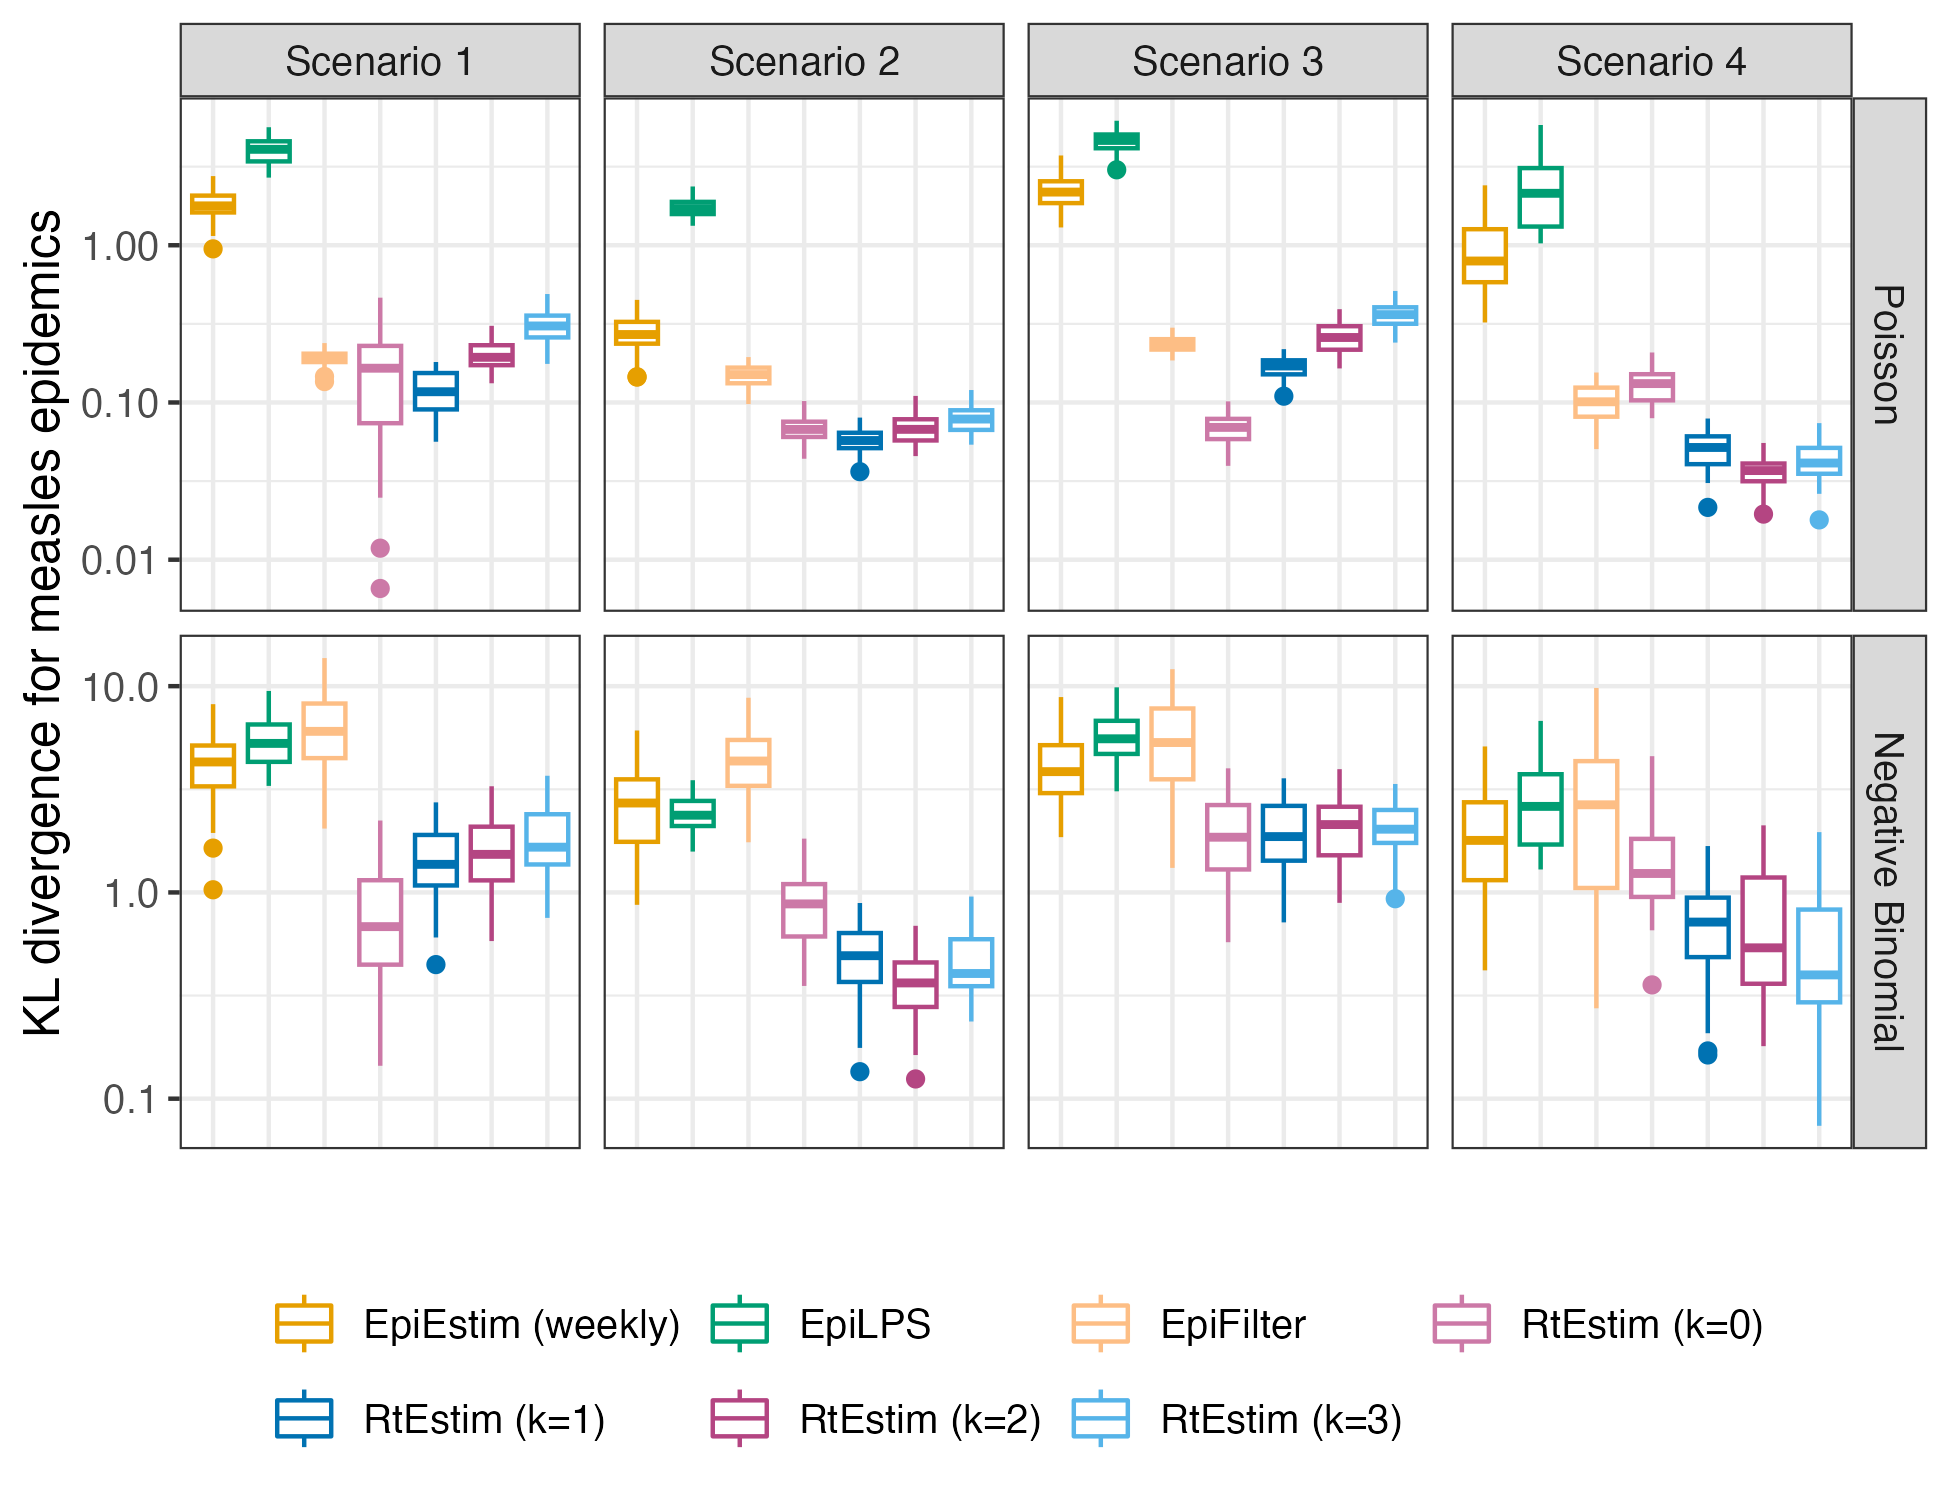
\includegraphics[width=1.0\linewidth]{fig/Fig3.png}
  \caption{{\bf Boxplot of mean KL divergence between $\hat{\calR}_t$ and true
  $\calR_t$ across 50 synthetic measles epidemics.} Performance of each approach given
  Poisson incidence is in top panels and negative binomial incidence is in bottom
  panels. The average excludes the first week in all settings, since
  \EpiEstim\ with a weekly sliding window does not provide estimates for the
  first week. Outliers beyond $1.5\times$IQR of each box are excluded for the
  sake of comparison with full range of the $y$-axis deferred to Figure A.3.1 in
  \nameref{S1_supp}.} 
  \label{fig:kl-res-measles}
\end{figure}

\begin{figure}[!t]
  \centering
  %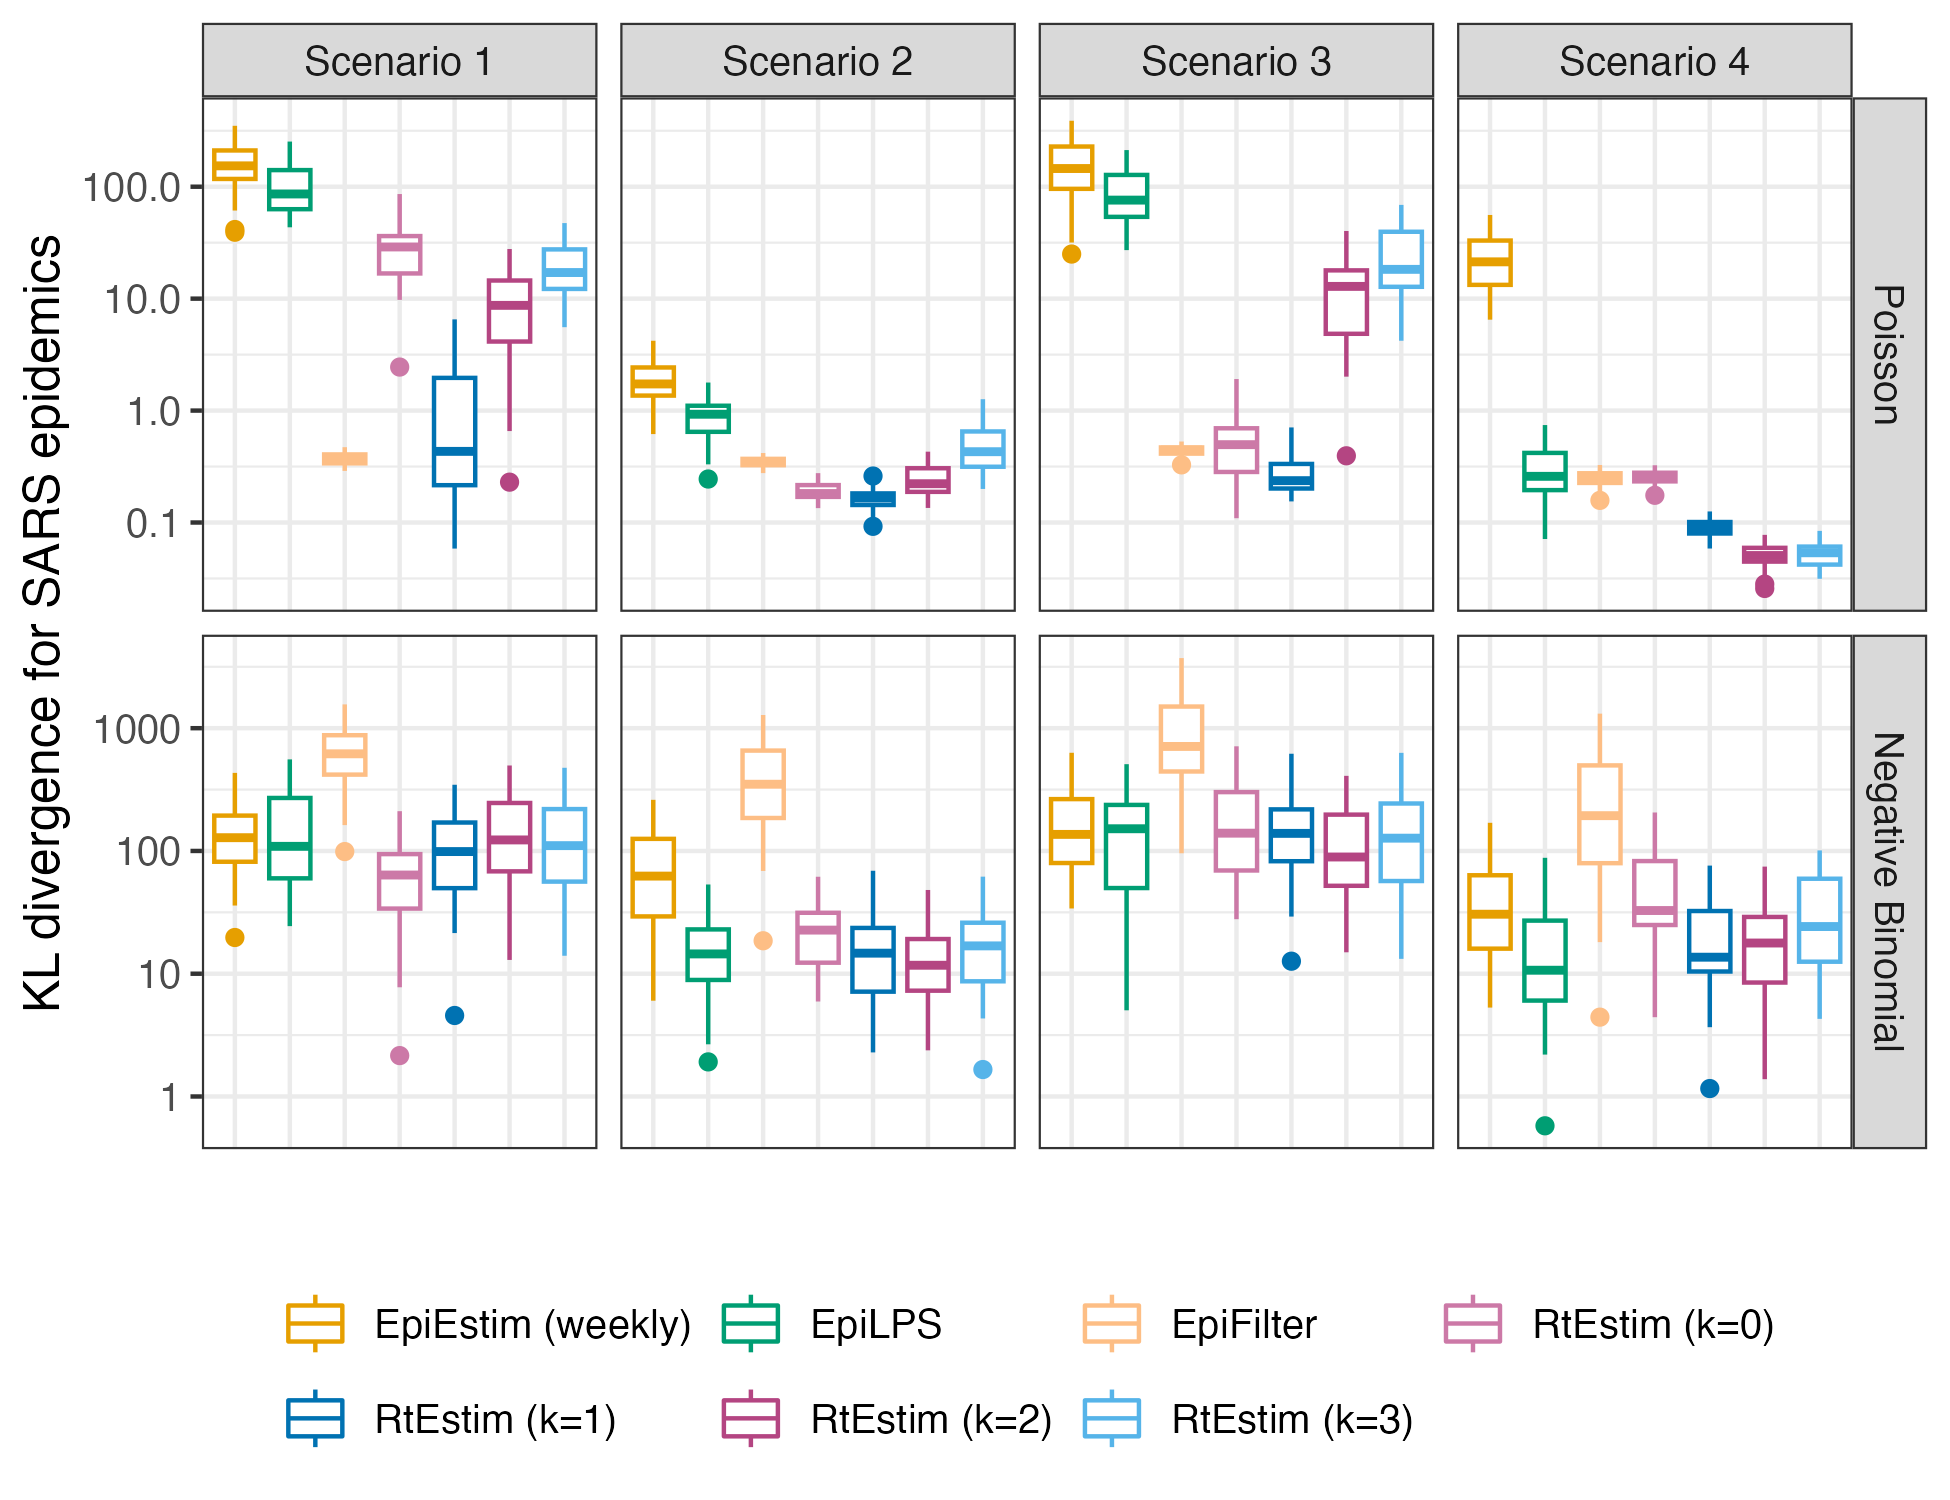
\includegraphics[width=1.0\linewidth]{fig/Fig4.png}
  \caption{{\bf Boxplot of mean KL divergence between $\hat{\calR}_t$ and true
  $\calR_t$ across 50 synthetic SARS epidemics.} Performance of each approach given Poisson
  incidence is in top panels and negative binomial incidence is in bottom panels. The
  average excludes the first week in all settings, since \EpiEstim\ with a
  weekly sliding window does not provide estimates for the first week. Outliers
  beyond $1.5\times$IQR of each box are excluded for the sake of comparison with
  full range of the $y$-axis deferred to Figure A.3.1 in \nameref{S1_supp}.} 
  \label{fig:kl-res-sars}
\end{figure}

\autoref{fig:pois-est-measles} shows one realization for the estimated
instantaneous reproduction number under the Poisson generative model in measles
synthetic epidemics for all four scenarios. An expanded visualization with each
estimated $\calR_t$ curve displayed in a separate panel is provided in Figure
A.6.1 in \nameref{S1_supp}. Ignoring the start of the epidemics, all methods look
accurate and recover the underlying curves well, except \EpiEstim\ with monthly
sliding windows, where the trajectories are shifted to the right. Compared to
\EpiEstim\ and \EpiLPS, which have rather severe difficulties at the beginning
of the period, \RtEstim\ and \EpiFilter\ estimates are more accurate without
suffering from the initialization problem. The edge problem in \EpiEstim\ and
\EpiLPS\ may be due to their priors, with the bias persisting for many days.
\RtEstim\ can also have edge problem though, it is less severe for smaller $k$.
Besides the edge problem, \EpiEstim\ (especially, with the monthly sliding
window) and \EpiLPS\ produce ``smooth'' estimated curves that are continuous at
the changepoints in Scenarios 1--3, resulting in large errors for a long period.
Since the piecewise constant \RtEstim\ estimator does not force any smoothness
in $\calR_t$, it easily captures the sharp change and nearly overlaps with the
true values in Scenario 1. \RtEstim\ with higher $k$ can work nearly as well due
to the $\ell_1$ penalty's ability to allow heterogenous smoothness. However,
similar to other methods, \RtEstim\ has some difficulty with the first few
timepoints, especially in the periodic scenario, where all methods fail to
capture the first peak with an accurately. \EpiFilter\ recovers the $\calR_t$
curves well in general, but tends to be more wiggly than other methods. 


\begin{figure}[!t]
  \centering
  %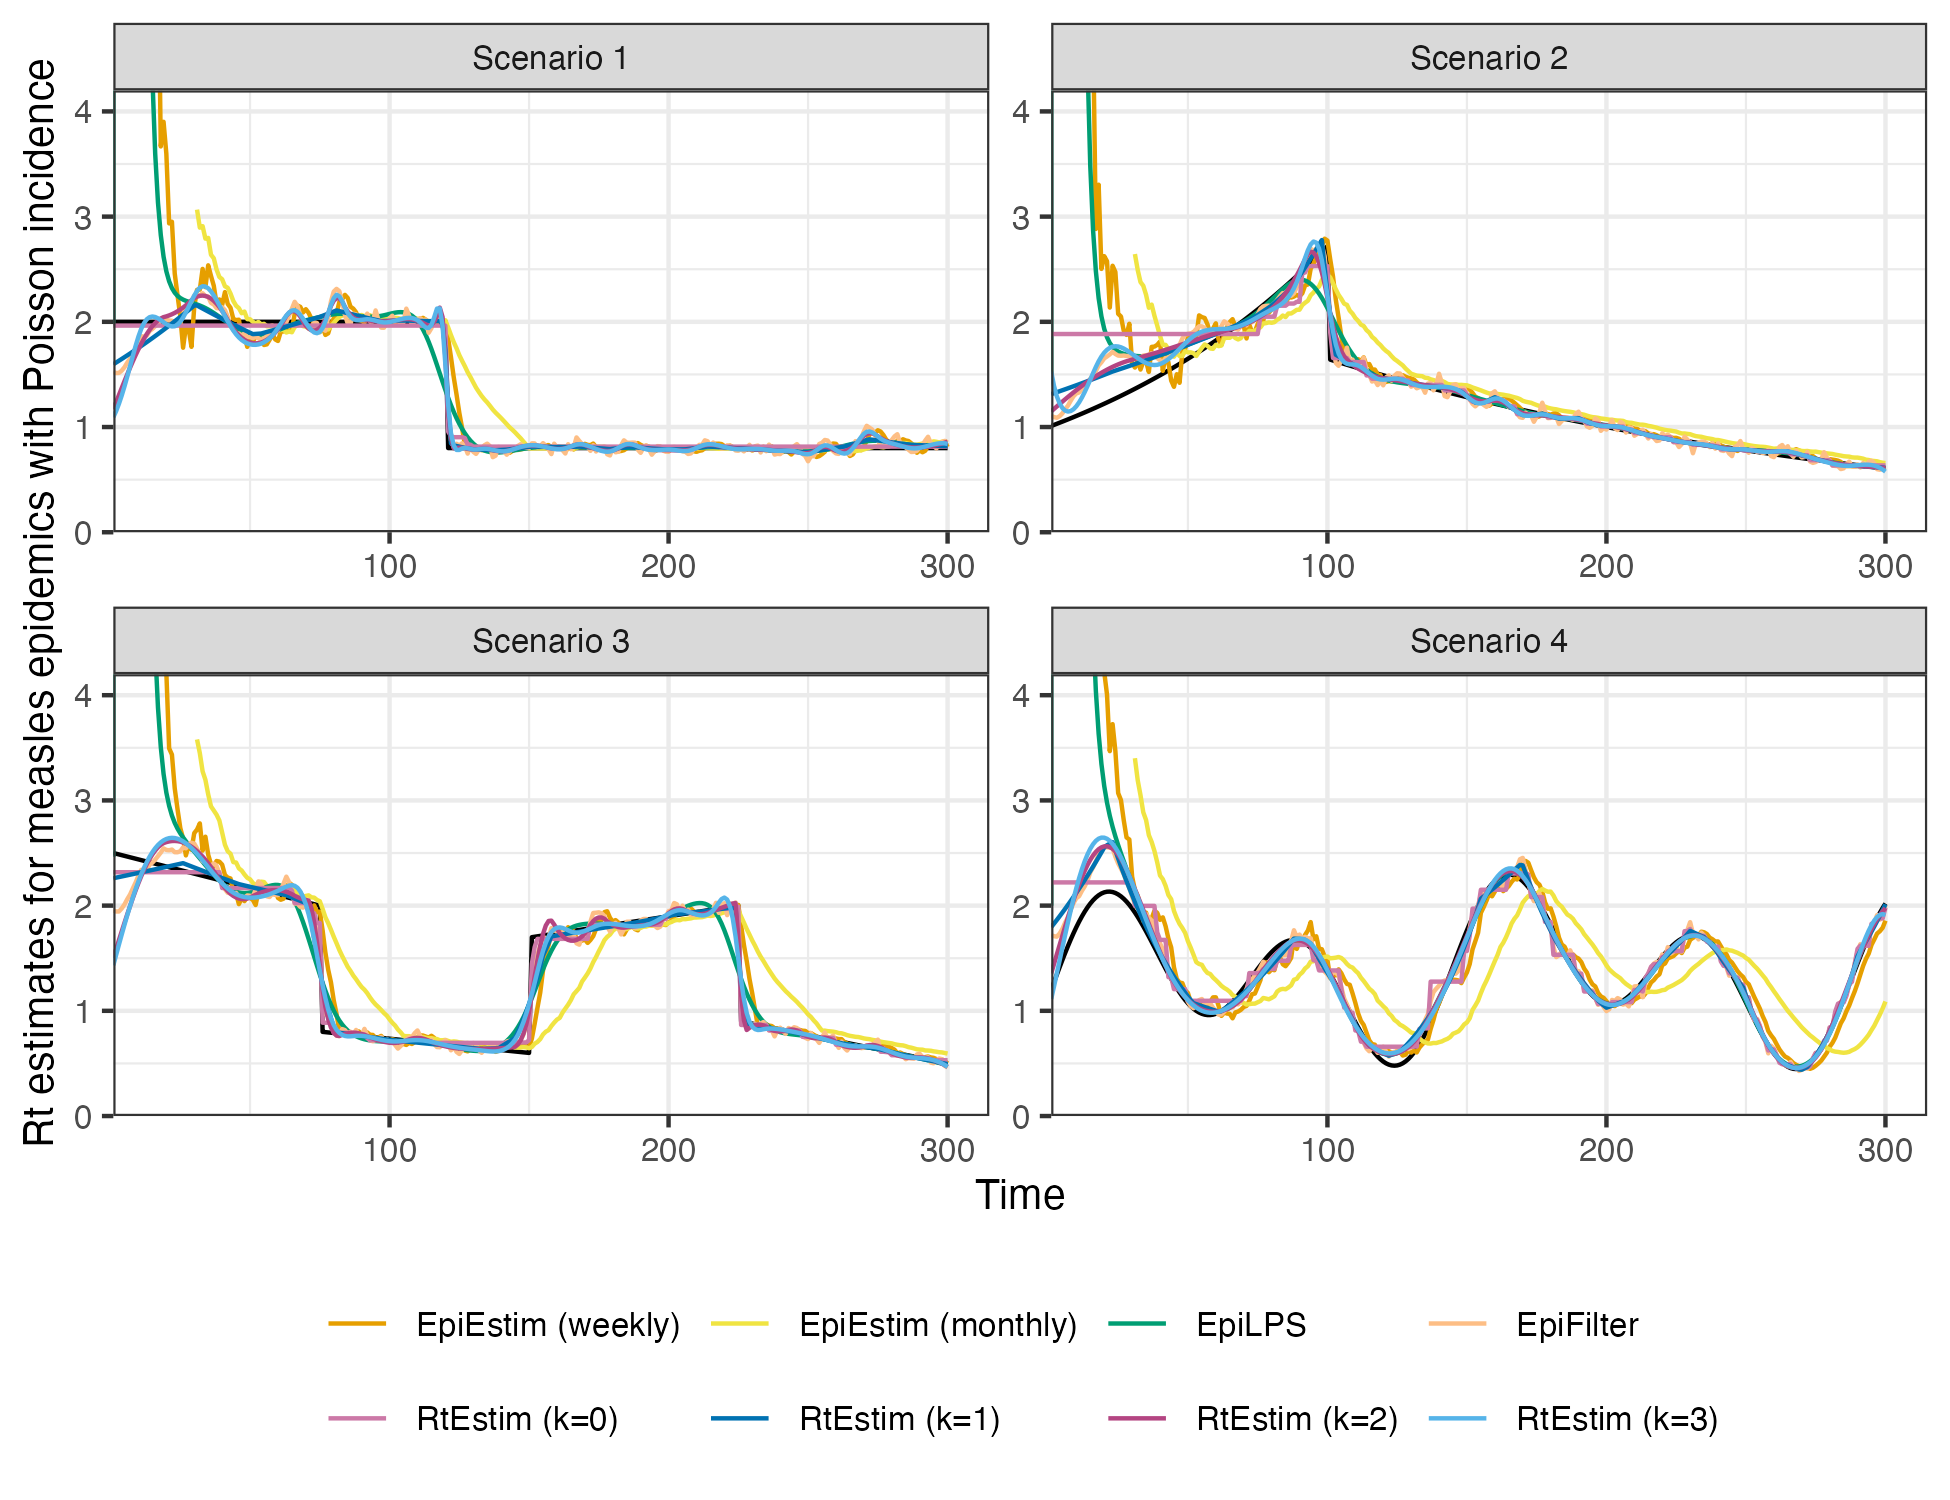
\includegraphics[width=1.0\linewidth]{fig/Fig5.png}
  \caption{{\bf $\calR_t$ estimates for realizations of a measles epidemic with
    Poisson observations.} An expanded visualization with each estimated
    $\calR_t$ curve displayed in a separate panel is provided in Figure A.6.1 in
    \nameref{S1_supp}.}
  \label{fig:pois-est-measles}
\end{figure}

\autoref{fig:nb-est-sars} is similar to \autoref{fig:pois-est-measles} but
shows estimated $\calR_t$ given negative binomial incidence in SARS epidemics
for each setting. An expanded visualization with each estimated $\calR_t$ curve
displayed in a separate panel is provided in Figure A.6.4 in \nameref{S1_supp}.
Compared to the \autoref{fig:pois-est-measles}, all methods perform worse
overall due to two main reasons: larger incidence and overdispersed data. All
methods are worse at the start of the epidemics. \EpiFilter\ is dramatically
wiggly. Our \RtEstim\ estimates are close to the best
performance in the first three $\calR_t$ scenarios, though they have
siginificant difficulties in the periodic scenario. 

\begin{figure}[!t]
  \centering
  %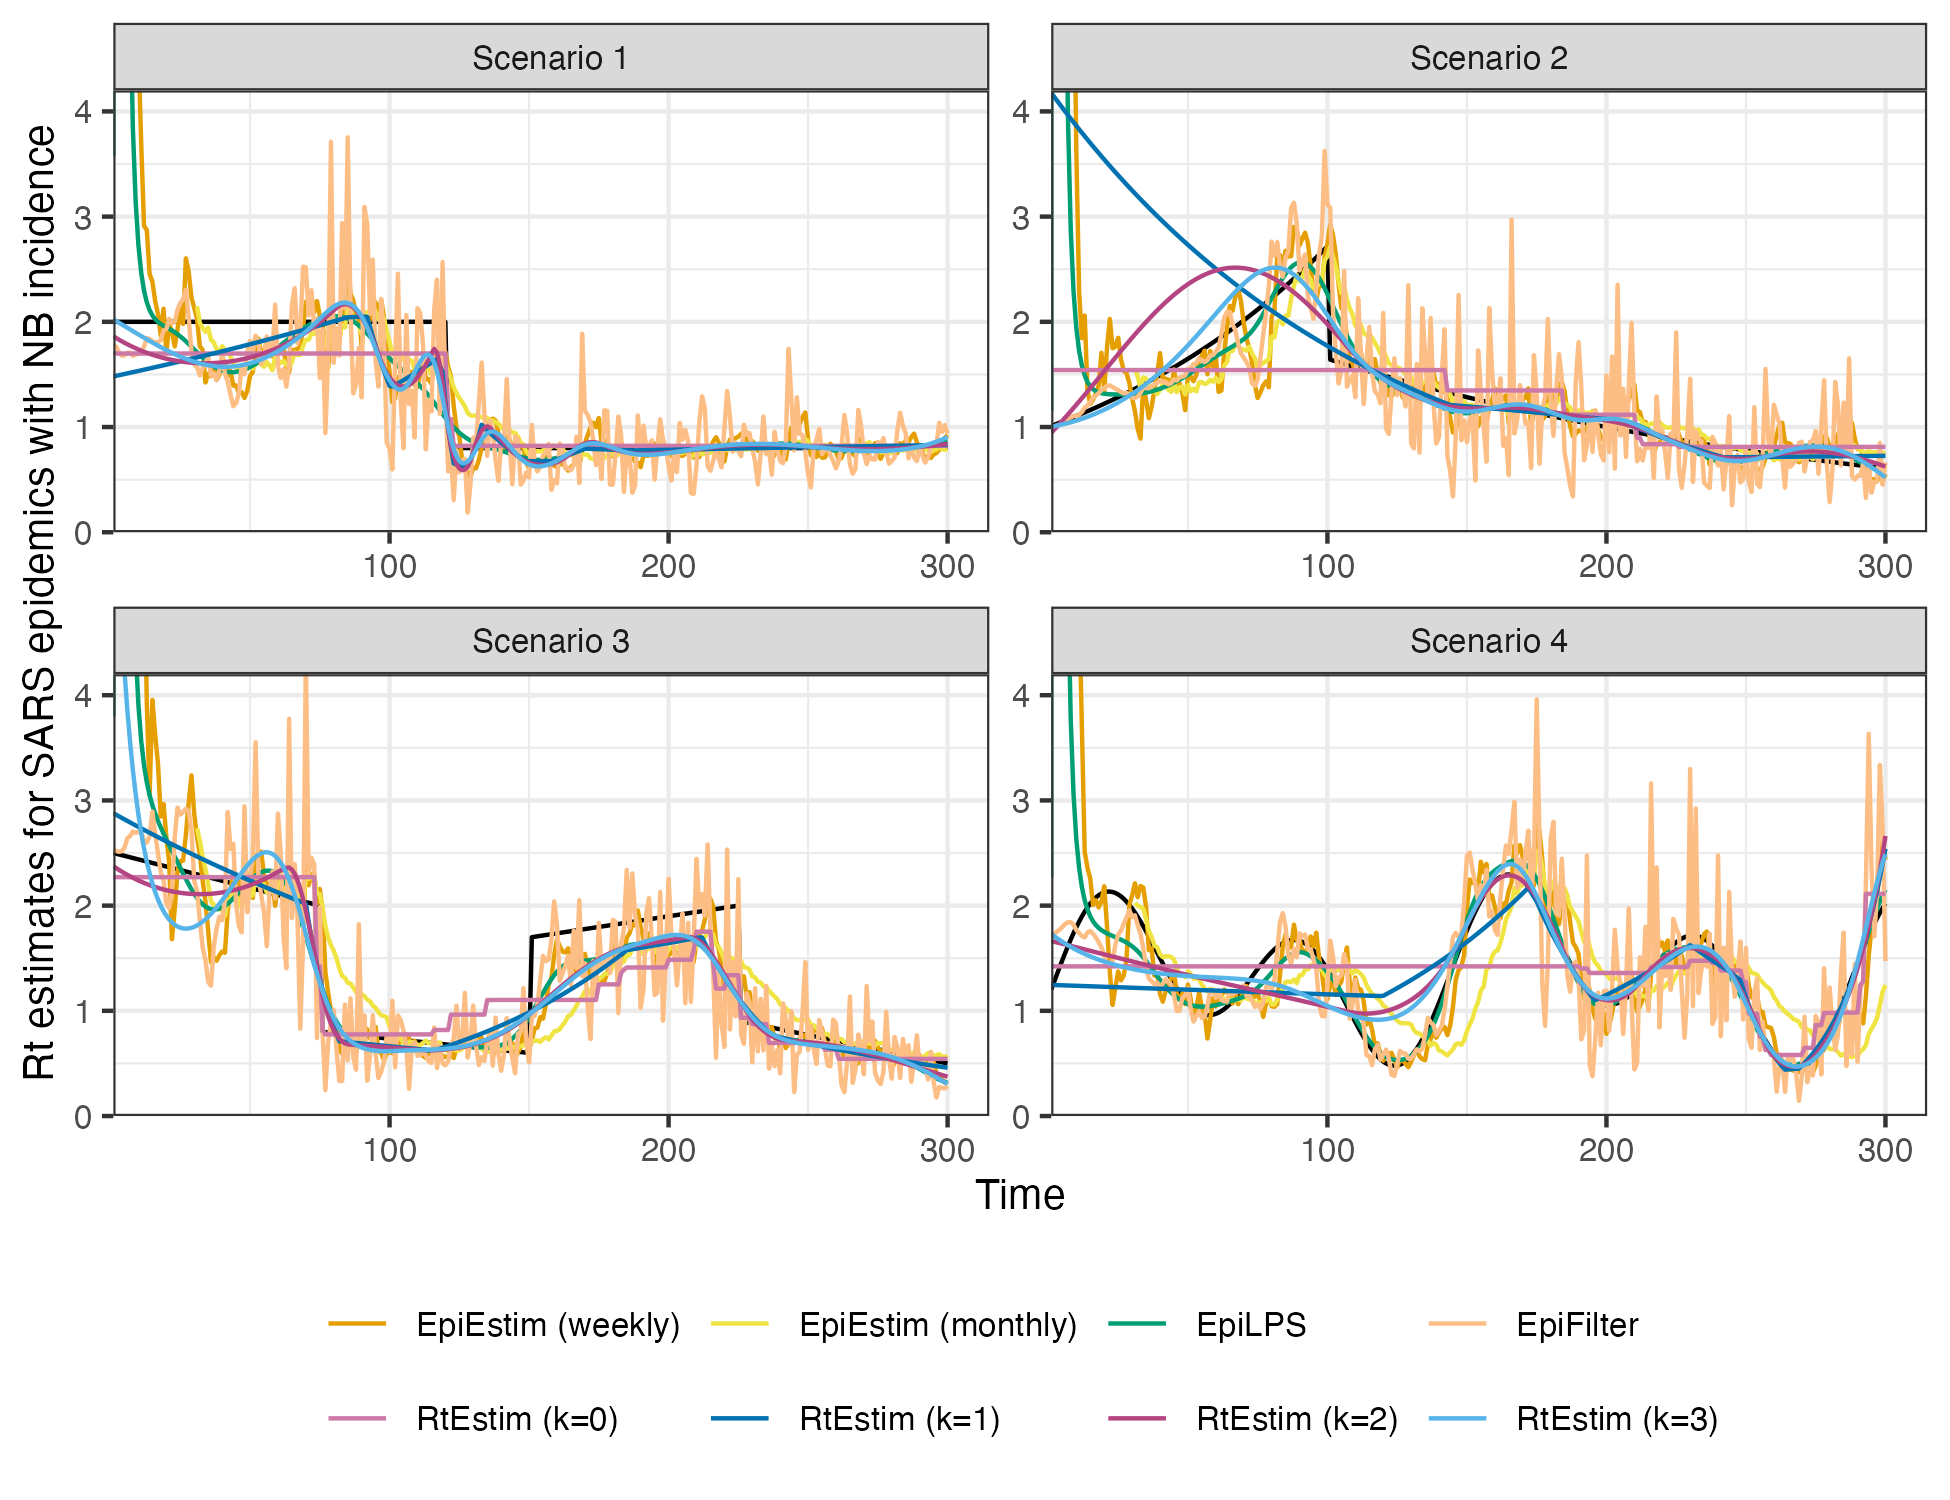
\includegraphics[width=1.0\linewidth]{fig/Fig6.png}
  \caption{
    {\bf $\calR_t$ estimates for realizations of a SARS epidemic with
    negative binomial observations.} An expanded visualization with each estimated
    $\calR_t$ curve displayed in a separate panel is provided in Figure A.6.4 in
    \nameref{S1_supp}.}
  \label{fig:nb-est-sars}
\end{figure}

Finally, it is important to provide a brief comparison of the running times of
all three models across the $8$ experimental settings. We find that almost all
models across all experiments complete within $10$ seconds. \RtEstim\ generally
takes the longest, due to a relatively large number of estimates---$50$ values
of $\lambda$ and $10$ folds of cross validation require $550$ estimates---while
other models run only a single time for a fixed setting of hyperparameters per
experiment. 


\subsection{Real-data results: Covid-19 incident cases in Canada}

We return to the data for Covid-19 confirmed incident cases in Canada examined
in \autoref{sec:intro}. In this section, we use the weighted average of the
serial interval distributions for the four dominant variants (shown in
\autoref{fig:intro-fig}) for the purposes of comparison with other methods, none
of which allow time-varying delays. The estimates for \RtEstim\ are displayed in
\autoref{fig:covid-rt} while the estimates of all competitors are deferred to
Figures A.8.1 and A.8.2 in \nameref{S1_supp}. 

Considering $k=1,2$ and 3, $\widehat{\calR}_t$ for Covid-19 in Canada is always
less than $2$ except at the very early stage, which means that one distinct
infected individual on average infects less than two other individuals in the
population. Examining three different settings for $k$, the temporal evolution
of $\widehat{\calR}$ (across all regularization levels $\lambda$) are similar
near the highest peak around the end of 2021 before dropping shortly thereafter.
Throughout the estimated curves, the peaks and troughs of the instantaneous
reproduction numbers precede the growth and decay cycles of confirmed cases, as
expected. We also visualize 95\% confidence bands for the point estimates with
$\lambda$ chosen by minimizing cross-validated KL divergence in
\autoref{fig:covid-rt}.     

\begin{figure}[!t]
  \centering
  %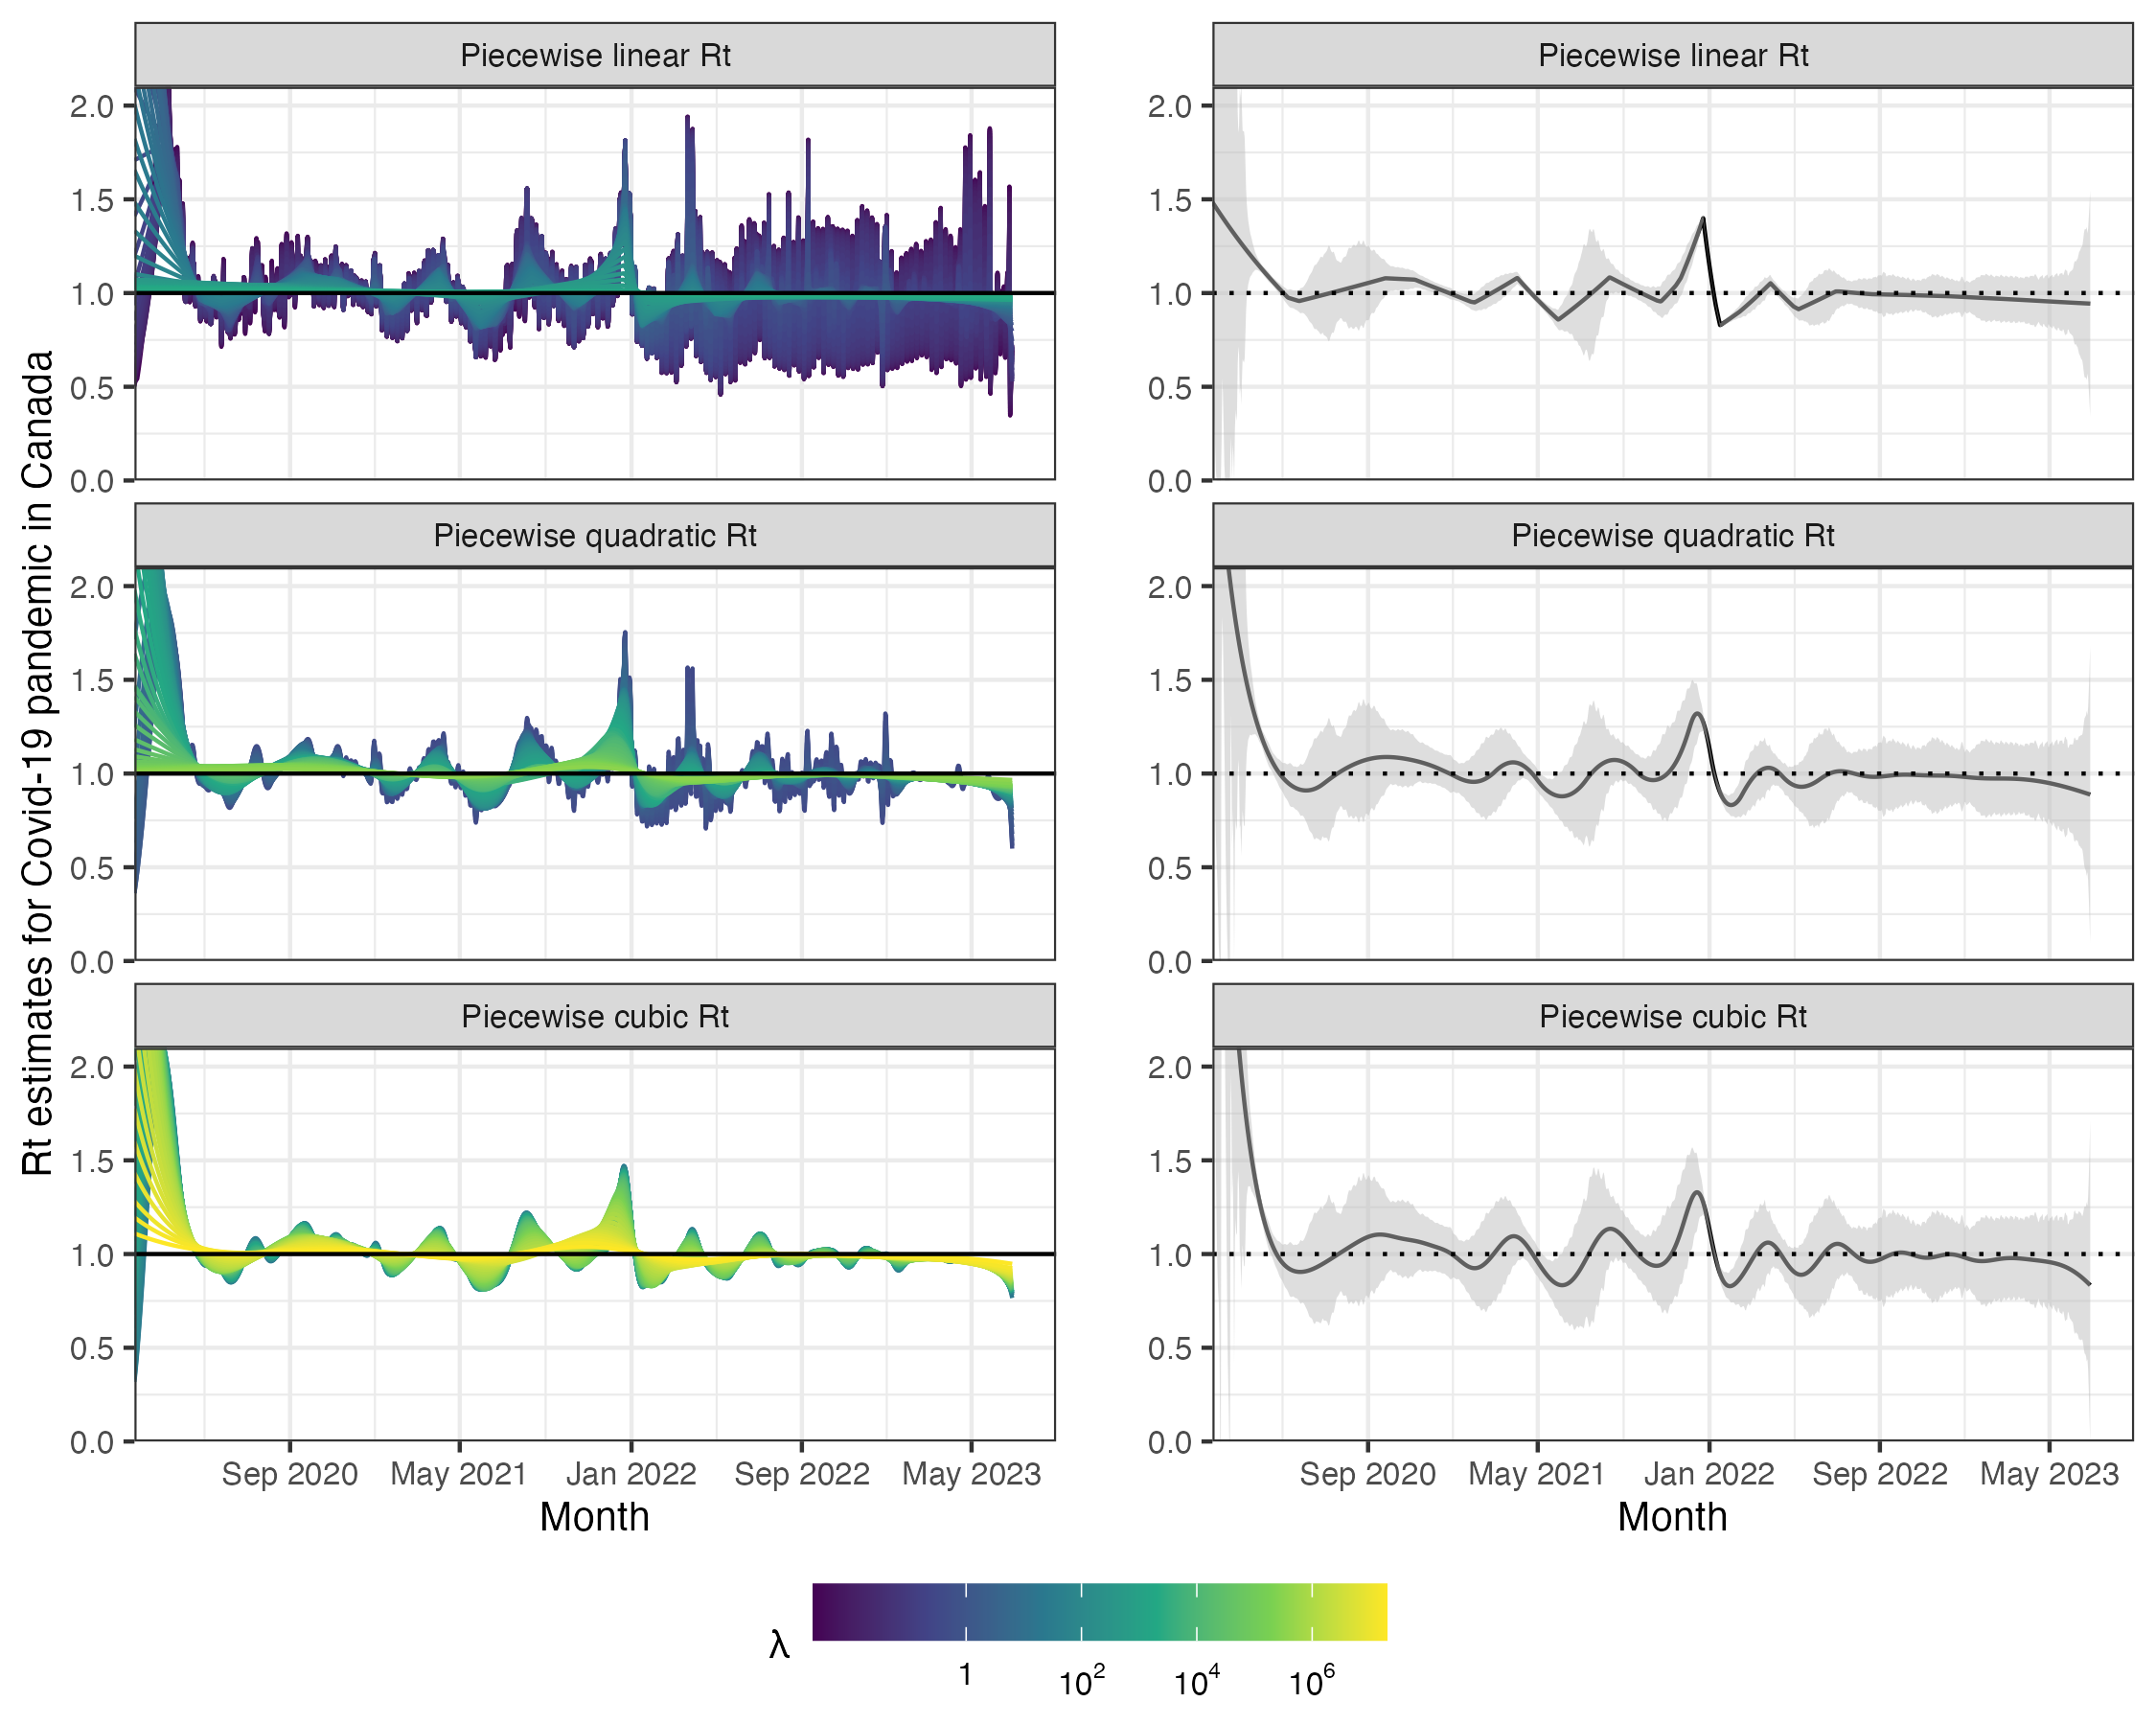
\includegraphics[width=1.0\linewidth]{fig/Fig7.png}
  \caption{{\bf Estimated instantaneous reproduction number based on Covid-19 daily
  confirmed incident cases.} The epidemic is between January 23rd, 2020 and June 28th, 2023 in
  Canada. The left panels show estimates corresponding to 50 tuning parameters.
  The right panels show the CV-tuned estimate along with approximate 95\%
  confidence bands. The top, middle and bottom panels show the estimated
  $\calR_t$ using the Poisson trend filtering in \eqref{eq:rt-ptf} with degrees
  $k=1,2,3$ respectively. All estimates use a constant serial interval
  distribution, which is the weighted sum of probabilities of the 4 dominant
  variants used in \autoref{fig:intro-fig}.}
  \label{fig:covid-rt}
\end{figure} 

The estimated instantaneous reproduction numbers are relatively unstable before
April, 2022. The highest peak coincides with the emergence and global spread of
the Omicron variant. The estimated instantaneous reproduction numbers fall below
1 during a few time periods, where the most obvious troughs are roughly from
April 2021 to July 2021 and from January, 2022 to April 2022. The first trough
coincides with the introduction of Covid-19 vaccines in Canada. The second
trough, shortly after the largest peak may be due to variety of factors
resulting in the depletion of the susceptible population such as increased
self-isolation in response to media coverage of the peak or immunity incurred
via recent infection. Since April 2022, the estimated instantaneous reproduction
number has remained relatively stable (fluctuating around one) corresponding to
low reported cases, though reporting behaviours also changed significantly since
the Omicron wave. 


\subsection{Real-data results: influenza in Baltimore, Maryland, 1918}

We also apply \RtEstim\ to daily reported influenza cases in Baltimore, Maryland
occurring during the world-wide pandemic of 1918 from September to November
\cite{frost1919influenza}. The data, shown in \autoref{fig:flu-dat}, is included
in the \EpiEstim\ \R\ package, along with the serial interval distribution. The
1918 influenza outbreak, caused by the H1N1 influenza A virus, was
unprecedentedly deadly with case fatality rate over 2.5\%, infecting almost
one-third of the population across the world \cite{taubenberger20061918}. The
CV-tuned piecewise cubic estimates in \autoref{fig:flu-res} better capture the
growth at the beginning of the pandemic in \autoref{fig:flu-dat}. The estimated
$\calR_t$ curve suggests that the transmissibility of the pandemic grew rapidly
over the first 30 days before declining below one after 50 days. However, it
also suggests an increase in infectiousness toward the end of the period. With
this data, it is difficult to determine if there is a second wave or a steady
decline ahead. The CV-tuned piecewise constant and linear estimates in
\autoref{fig:flu-res} both suggest a steady decline. This conclusion is
supported by the fact that incident cases decline to zero at the end of the
period, matching $\calR_t$ estimates in \cite{cori2013new}, which are all lower
than one. Results from alternative software is deferred to Figures A.8.3 and
A.8.4 in \nameref{S1_supp}.

\begin{figure}[!t]
  \centering
  %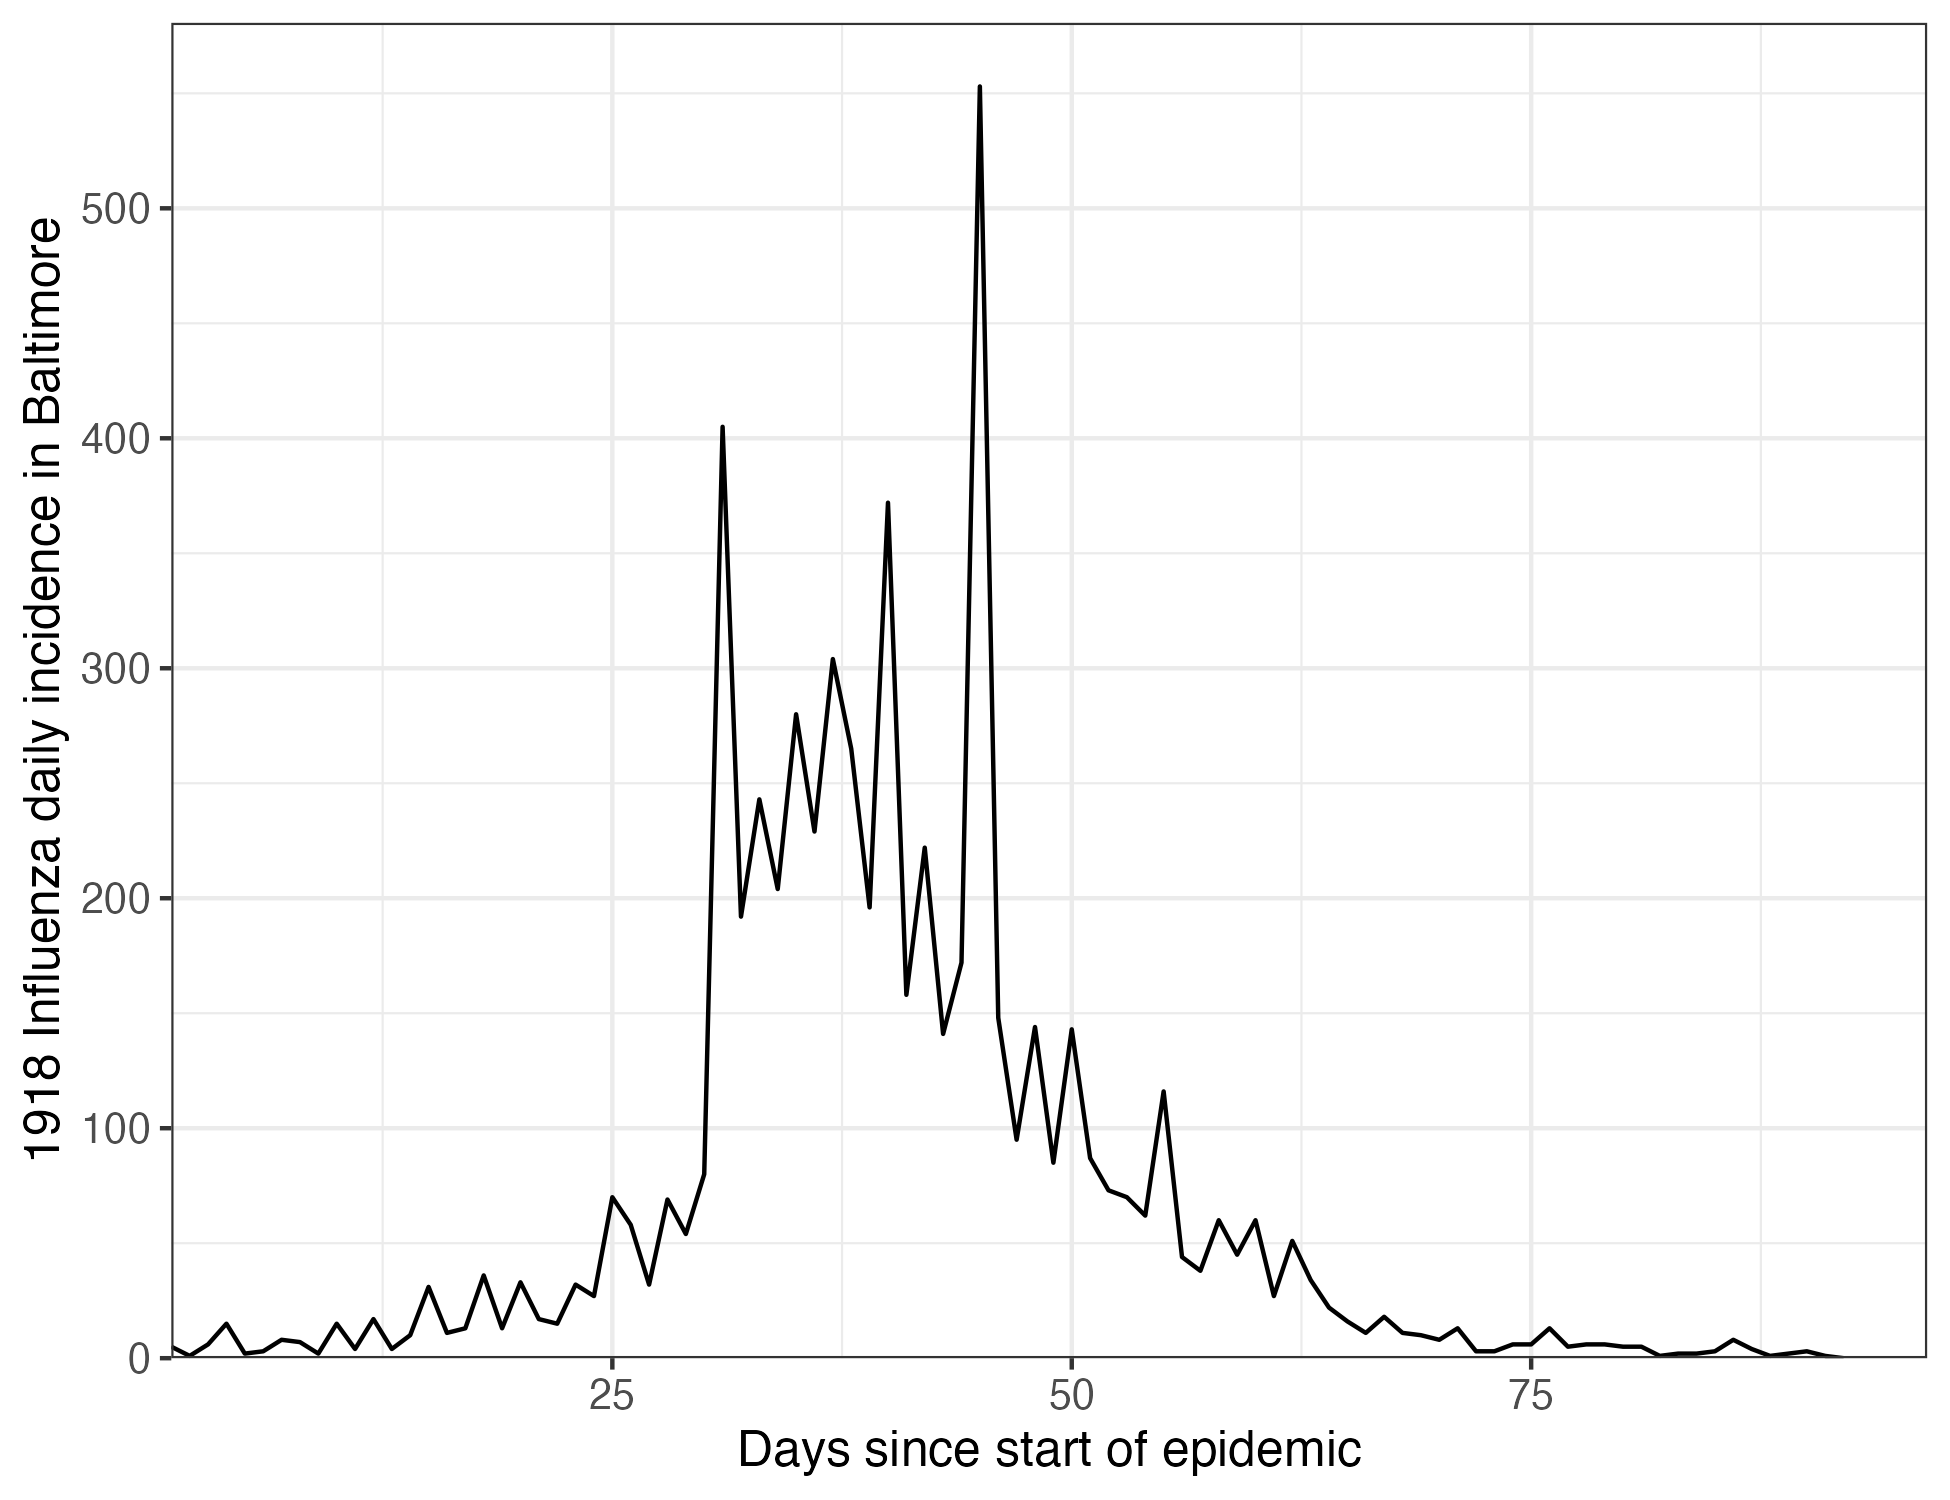
\includegraphics[width=1.0\linewidth]{fig/Fig8.png}
  \caption{{\bf Daily incident influenza cases in Baltimore, Maryland between September 
  and November 1918.}} 
  \label{fig:flu-dat}
\end{figure} 

\begin{figure}[!t]
  \centering
  %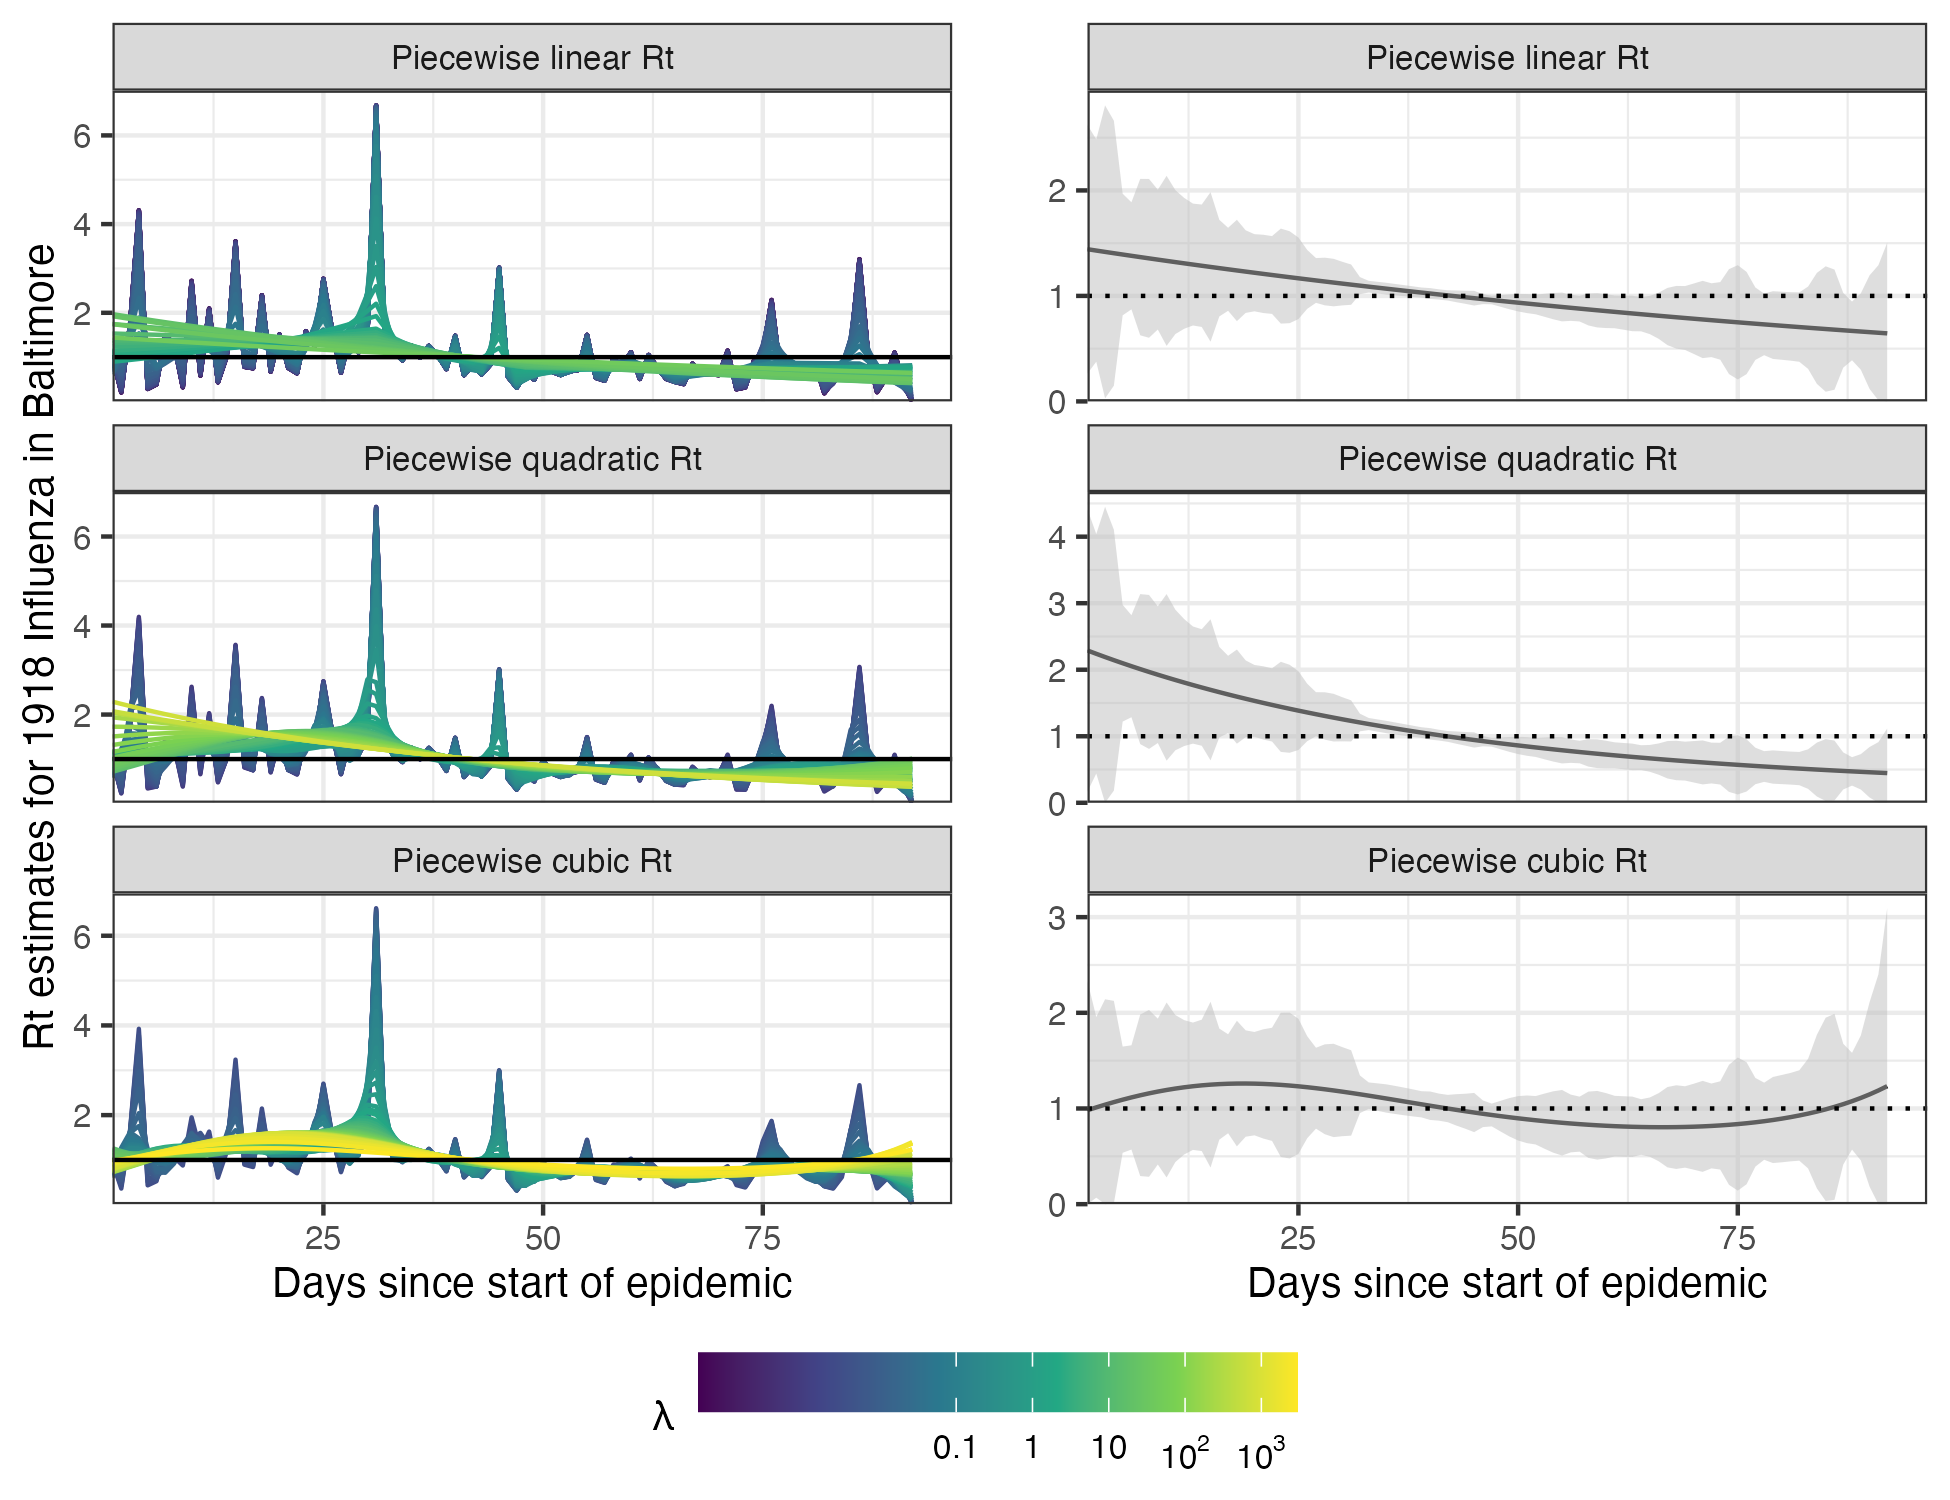
\includegraphics[width=1.0\linewidth]{fig/Fig9.png}
  \caption{{\bf Estimated instantaneous reproduction numbers for influenza in
  Baltimore, Maryland in 1918.} The left panels show estimates for a set of 50
  tuning parameters. The right column displays the CV-tuned estimates with
  approximate 95\% confidence bands. The rows (top to bottom) show $\hat\calR_t$
  using Poisson trend filtering with $k=1,2,3$
  respectively.} 
  \label{fig:flu-res}
\end{figure} 


\section{Discussion}
\label{sec:disc}

The \RtEstim\ methodology provides a locally adaptive estimator using Poisson
trend filtering. It captures the heterogeneous smoothness of instantaneous
reproduction numbers given observed incidence data rather than resulting in
global smoothness. This is a nonparametric regression model which can be written
as a convex optimization problem. Minimizing the negative logliklihood of
observations guarantees data fidelity while the penalty on divided differences
between pairs of neighbouring parameters imposes smoothness. The
$\ell_1$-regularization results in sparsity of the divided differences,
leading to heterogeneous smoothness across time. 


The property of local adaptivity (heterogenous smoothness) is useful to
automatically distinguish, for example, seasonal outbreaks from outbreaks driven
by other factors (behavioural changes, foreign introduction, etc.). Given a
well-chosen polynomial degree, the growth rates can be quickly detected,
potentially advising public health authorities to implement policy changes. The
instantaneous reproduction numbers can be estimated retrospectively to examine
the efficacy of such policies, whether they result in $\calR_t$ falling below 1
or the speed of their effects. The smoothness of $\calR_t$ curves (including the
polynomial degrees and tuning parameters) should be chosen based on the purpose
of the study in practice or with data-driven risk estimation by cross validation. 


Our method provides a natural way to deal with missing data, for example, on
weekends and holidays or due to changes in reporting frequency. While solving
the convex optimization problem, our method can easily handle uneven spacing or
irregular reporting. Computing the total primary infectiousness is also easily
generalized to irregular reporting through automatic modifications of the
discretization of the serial interval distribution. However, there are many
other aspects to be considered in choosing the delay distribution to improve
accuracy \cite{park2024estimating}. Additionally, because the $\ell_1$ penalty
introduces sparsity (operating like a median rather than a mean), this procedure
is relatively insensitive to spurious outliers compared to $\ell_2$
regularization. 


There are a number of limitations that may influence the quality of $\calR_t$
estimation. While our model is generic for incidence data rather than tailored
to any specific disease, it does assume that the generation interval is short
relative to the period of data collection. More specialized methodologies would
be required for diseases with long incubation periods such as HIV or Hepatitis.
Our approach, does not explicitly model imported cases, nor distinguish between
subpopulations that may have different mixing behaviour. However, a natural
extension to handle imported cases is to follow the suggested procedure of
\cite{thompson2019improved}. By including imported cases only in $\eta_t$ rather
than in both $y_t$ and $\eta_t$, we exclude individuals who were infected
elsewhere, lowering $\calR_t$, but correctly reflecting the number of new
primary infectees.

While the Poisson assumption is common, it does not handle overdispersion
(observation variance larger than the mean). The negative binomial distribution
is a good alternative, but more difficult to estimate in this context. As
described in \autoref{sec:intro}, the expression for $\calR$ assumes that a
relatively constant proportion of true infections is reported. However, if this
proportion varies with time (say, due to changes in surveillance practices or
testing recommendations), the estimates may be biased over this window. A good
example is in early January 2022, during the height of the Omicron wave, Canada
moved from testing all symptomatic individuals to testing only those in at-risk
groups. The result was a sudden change that would render $\calR_t$ estimates on
either side of this timepoint incommensurable.


Our \RtEstim\ implementation can take a fixed serial interval throughout the
period of study (as implemented in simulation and in the real epidemics) or 
use time-varying serial interval distributions (as implemented 
in \autoref{fig:intro-fig} for Covid-19 data in Canada). In reality, the serial
interval may vary due to changes in the factors such as population immunity 
\cite{nash2023estimating}. One issue regarding the serial interval distribution 
relates to equating serial and generation intervals (also mentioned above). 
The serial interval distribution is generally wider than that 
of the generation interval, because the serial interval involves the convolution
of two distributions, and is unlikely to actually follow a named distribution
like gamma, though it may be reasonably well approximated by one. Our
implementation allows for an arbitrary distribution to be used, but requires the
user to specify the discretization explicitly, requiring more nuanced knowledge
than is typically available. Pushing this analysis further, to accommodate other
types of incidence data (hospitalizations or deaths), a modified generation
interval distribution would be necessary, and further assumptions would be
required as well. Or else, one would first need to deconvolve deaths to
infection onset before using our software.


Accurate statistical coverage of a function is a difficult problem, and the
types of (frequentist) guarantees that can be made are not always what one would
want \cite{genovese2008adaptive}. We examine the coverage of our approximate
confidence interval in simulation, with details are deferred to Section A.6 in
\nameref{S1_supp}. Empirically, our observations for our method, as well as all
others we have seen, follow a similar (undesirable) pattern: when
$\mathcal{R}_t$ is stable, they over cover dramatically (even implausibly narrow
intervals have 100\% coverage); but when $\mathcal{R}_t$ changes abruptly, they
under cover. Theoretically, whether these intervals should be expected to
provide $(1-\alpha)\%$ coverage simultaneously over all time while being narrow
enough to provide useful uncertainty quantification is neither easy nor settled.
An alternative to our approximation in \autoref{sec:conf-band}, which we defer
to future work, is to use the data fission method proposed by
\cite{leiner2023data}, which provides post-selection inference for trend
filtering.


Nonetheless, our methodology is implemented in a lightweight \R\ package
\texttt{rtestim} and computed efficiently, especially for large-scale data, with
a proximal Newton solver coded in \cpp. Given available incident case data,
prespecified serial interval distribution, and a choice of degree $k$, \RtEstim\
is able to produce accurate estimates of instantaneous reproduction number and
provide efficient tuning parameter selection via cross validation. 

\section*{Supporting information}

\paragraph*{S1 Appendix.}
\label{S1_supp}

{\bf Supplement for RtEstim: Time-varying reproduction number estimation with trend filtering.} 
This includes eight sections, Sections A.1--A.8. Section A.1: Derivation of Kullback Leibler divergence for accuracy comparison. 
Section A.2: Supplmentary details on experimental settings.
Section A.3: Supplementary experimental results on accuracy comparison.
Section A.4: Experimental results on accuracy under misspecification of serial interval distributions.
Section A.5: Time comparisons of all methods.
Section A.6: Confidence interval coverage.
Section A.7: Data examples and alternative visualizations of Figs 5 and 6.
Section A.8: Application of RtEstim and all competitors on real epidemics.

\section*{Acknowledgments}

This research was enabled in part by support provided by 
BC DRI group who manages Cedar cloud (https://docs.alliancecan.ca/wiki/Cedar)
and the Digital Research Alliance of Canada (alliancecan.ca).

\nolinenumbers


\begin{thebibliography}{10}

  \bibitem{nishiura2009effective}
  Nishiura H, Chowell G.
  \newblock The effective reproduction number as a prelude to statistical
    estimation of time-dependent epidemic trends.
  \newblock Mathematical and statistical estimation approaches in epidemiology.
    2009; p. 103--121.
  
  \bibitem{fraser2007estimating}
  Fraser C.
  \newblock Estimating individual and household reproduction numbers in an
    emerging epidemic.
  \newblock PloS one. 2007;2(8):e758.
  
  \bibitem{gostic2020practical}
  Gostic KM, McGough L, Baskerville EB, Abbott S, Joshi K, Tedijanto C, et~al.
  \newblock Practical considerations for measuring the effective reproductive
    number, \emph{R}$_t$.
  \newblock PLoS Computational Biology. 2020;16(12):e1008409.
  
  \bibitem{anderson1991infectious}
  Anderson RM, May RM.
  \newblock Infectious diseases of humans: dynamics and control.
  \newblock Oxford university press. 1991.
  
  \bibitem{wallinga2004different}
  Wallinga J, Teunis P.
  \newblock Different epidemic curves for severe acute respiratory syndrome
    reveal similar impacts of control measures.
  \newblock American Journal of epidemiology. 2004;160(6):509--516.
  
  \bibitem{hao2020reconstruction}
  Hao X, Cheng S, Wu D, Wu T, Lin X, Wang C.
  \newblock Reconstruction of the full transmission dynamics of COVID-19 in
    Wuhan.
  \newblock Nature. 2020;584(7821):420--424.
  
  \bibitem{goldstein2023semiparametric}
  Goldstein IH, Parker DM, Jiang S, Minin VM.
  \newblock Semiparametric inference of effective reproduction number dynamics
    from wastewater pathogen surveillance data.
  \newblock arXiv preprint arXiv:230815770. 2023.
  
  \bibitem{goldstein2024incorporating}
  Goldstein IH, Wakefield J, Minin VM.
  \newblock Incorporating testing volume into estimation of effective
    reproduction number dynamics.
  \newblock Journal of the Royal Statistical Society Series A: Statistics in
    Society. 2024;187(2):436--453.
  
  \bibitem{cori2020package}
  Cori A, Cauchemez S, Ferguson NM, Fraser C, Dahlqwist E, Demarsh PA, et~al..
    {EpiEstim}: estimate time varying reproduction numbers from epidemic curves.
    2020.
  
  \bibitem{cori2013new}
  Cori A, Ferguson NM, Fraser C, Cauchemez S.
  \newblock A new framework and software to estimate time-varying reproduction
    numbers during epidemics.
  \newblock American Journal of Epidemiology. 2013;178(9):1505--1512.
  
  \bibitem{thompson2019improved}
  Thompson RN, Stockwin JE, van Gaalen RD, Polonsky JA, Kamvar ZN, Demarsh PA,
    et~al.
  \newblock Improved inference of time-varying reproduction numbers during
    infectious disease outbreaks.
  \newblock Epidemics. 2019;29:100356.
  
  \bibitem{nash2023estimating}
  Nash RK, Bhatt S, Cori A, Nouvellet P.
  \newblock Estimating the epidemic reproduction number from temporally
    aggregated incidence data: A statistical modelling approach and software
    tool.
  \newblock PLoS Computational Biology. 2023;19(8):e1011439.
  
  \bibitem{abbott2020estimating}
  Abbott S, Hellewell J, Thompson RN, Sherratt K, Gibbs HP, Bosse NI, et~al.
  \newblock Estimating the time-varying reproduction number of {SARS-CoV-2} using
    national and subnational case counts.
  \newblock Wellcome Open Research. 2020;5:112.
  
  \bibitem{EpiNow2}
  Abbott S, Funk S, Hickson J, Badr HS, Monticone P, Ellis P, et~al..
    epiforecasts/{EpiNow2}: 1.4.0 release; 2023.
  
  \bibitem{lison2024generative}
  Lison A, Abbott S, Huisman J, Stadler T.
  \newblock Generative {B}ayesian modeling to nowcast the effective reproduction
    number from line list data with missing symptom onset dates.
  \newblock PLoS Computational Biology. 2024;20(4):e1012021.
  
  \bibitem{parag2021improved}
  Parag KV.
  \newblock Improved estimation of time-varying reproduction numbers at low case
    incidence and between epidemic waves.
  \newblock PLoS Computational Biology. 2021;17(9):e1009347.
  
  \bibitem{gressani2022epilps}
  Gressani O, Wallinga J, Althaus CL, Hens N, Faes C.
  \newblock EpiLPS: A fast and flexible {B}ayesian tool for estimation of the
    time-varying reproduction number.
  \newblock PLoS Computational Biology. 2022;18(10):e1010618.
  
  \bibitem{trevisin2023spatially}
  Trevisin C, Bertuzzo E, Pasetto D, Mari L, Miccoli S, Casagrandi R, et~al.
  \newblock Spatially explicit effective reproduction numbers from incidence and
    mobility data.
  \newblock Proceedings of the National Academy of Sciences.
    2023;120(20):e2219816120.
  
  \bibitem{abry2020spatial}
  Abry P, Pustelnik N, Roux S, Jensen P, Flandrin P, Gribonval R, et~al.
  \newblock Spatial and temporal regularization to estimate {COVID-19}
    reproduction number \emph{R(t)}: Promoting piecewise smoothness via convex
    optimization.
  \newblock PLoS ONE. 2020;15(8):e0237901.
  
  \bibitem{pascal2022nonsmooth}
  Pascal B, Abry P, Pustelnik N, Roux S, Gribonval R, Flandrin P.
  \newblock Nonsmooth convex optimization to estimate the {C}ovid-19 reproduction
    number space-time evolution with robustness against low quality data.
  \newblock IEEE Transactions on Signal Processing. 2022;70:2859--2868.
  
  \bibitem{pircalabelu2023spline}
  Pircalabelu E.
  \newblock A spline-based time-varying reproduction number for modelling
    epidemiological outbreaks.
  \newblock Journal of the Royal Statistical Society Series C: Applied
    Statistics. 2023;72(3):688--702.
  
  \bibitem{ho2023accounting}
  Ho F, Parag KV, Adam DC, Lau EH, Cowling BJ, Tsang TK.
  \newblock Accounting for the Potential of Overdispersion in Estimation of the
    Time-varying Reproduction Number.
  \newblock Epidemiology. 2023;34(2):201--205.
  
  \bibitem{azmon2014estimation}
  Azmon A, Faes C, Hens N.
  \newblock On the estimation of the reproduction number based on misreported
    epidemic data.
  \newblock Statistics in Medicine. 2014;33(7):1176--1192.
  
  \bibitem{gressani2021approximate}
  Gressani O, Faes C, Hens N.
  \newblock An approximate {B}ayesian approach for estimation of the
    instantaneous reproduction number under misreported epidemic data.
  \newblock Biometrical Journal. 2022;65(6):2200024.
  
  \bibitem{jin2023epimix}
  Jin S, Dickens BL, Lim JT, Cook AR.
  \newblock {EpiMix}: A novel method to estimate effective reproduction number.
  \newblock Infectious Disease Modelling. 2023;8(3):704--716.
  
  \bibitem{hettinger2023estimating}
  Hettinger G, Rubin D, Huang J.
  \newblock Estimating the instantaneous reproduction number with imperfect data:
    a method to account for case-reporting variation and serial interval
    uncertainty.
  \newblock arXiv preprint arXiv:230212078. 2023.
  
  \bibitem{CovidTimelineCanada}
  Berry I, O'Neill M, Sturrock SL, Wright JE, Acharya K, Brankston G, et~al.
  \newblock A sub-national real-time epidemiological and vaccination database for
    the {COVID}-19 pandemic in Canada.
  \newblock Scientific Data. 2021;8(1):{10.1038/s41597-021-00955-2}.
  
  \bibitem{duotang_2023}
  Coronavirus Variants Rapid Response Network Computational~Analysis M, Group
    EOC. CoVaRR-NET/duotang: Release for Zenodo Archive; 2023.
  \newblock Available from: \url{https://doi.org/10.5281/zenodo.10367461}.
  
  \bibitem{xu2023assessing}
  Xu X, Wu Y, Kummer AG, Zhao Y, Hu Z, Wang Y, et~al.
  \newblock Assessing changes in incubation period, serial interval, and
    generation time of SARS-CoV-2 variants of concern: a systematic review and
    meta-analysis.
  \newblock BMC medicine. 2023;21(1):374.
  
  \bibitem{park2021forward}
  Park SW, Sun K, Champredon D, Li M, Bolker BM, Earn DJ, et~al.
  \newblock Forward-looking serial intervals correctly link epidemic growth to
    reproduction numbers.
  \newblock Proceedings of the National Academy of Sciences.
    2021;118(2):e2011548118.
  
  \bibitem{pitzer2021impact}
  Pitzer VE, Chitwood M, Havumaki J, Menzies NA, Perniciaro S, Warren JL, et~al.
  \newblock The impact of changes in diagnostic testing practices on estimates of
    {COVID-19} transmission in the {U}nited {S}tates.
  \newblock American Journal of Epidemiology. 2021;190(9):1908--1917.
  
  \bibitem{hitchings2021usefulness}
  Hitchings MD, Dean NE, Garc{\'\i}a-Carreras B, Hladish TJ, Huang AT, Yang B,
    et~al.
  \newblock The usefulness of the test-positive proportion of severe acute
    respiratory syndrome coronavirus 2 as a surveillance tool.
  \newblock American Journal of Epidemiology. 2021;190(7):1396--1405.
  
  \bibitem{pellis2021challenges}
  Pellis L, Scarabel F, Stage HB, Overton CE, Chappell LH, Fearon E, et~al.
  \newblock Challenges in control of {COVID-19}: short doubling time and long
    delay to effect of interventions.
  \newblock Philosophical Transactions of the Royal Society B.
    2021;376(1829):20200264.
  
  \bibitem{EALES2024100742}
  Eales O, Riley S.
  \newblock Differences between the true reproduction number and the apparent
    reproduction number of an epidemic time series.
  \newblock Epidemics. 2024;46:100742.
  
  \bibitem{park2024estimating}
  Park SW, Akhmetzhanov AR, Charniga K, Cori A, Davies NG, Dushoff J, et~al.
  \newblock Estimating epidemiological delay distributions for infectious
    diseases.
  \newblock medRxiv. 2024; p. 2024--01.
  
  \bibitem{kim2009ell_1}
  Kim SJ, Koh K, Boyd S, Gorinevsky D.
  \newblock $\ell_1$ trend filtering.
  \newblock SIAM Review. 2009;51(2):339--360.
  
  \bibitem{tibshirani2014adaptive}
  Tibshirani RJ.
  \newblock Adaptive piecewise polynomial estimation via trend filtering.
  \newblock The Annals of Statistics. 2014;42(1):285--323.
  
  \bibitem{tibshirani2022divided}
  Tibshirani RJ.
  \newblock Divided differences, falling factorials, and discrete splines:
    Another look at trend filtering and related problems.
  \newblock Foundations and Trends in Machine Learning.
    2022;15(6):694--846.
  
  \bibitem{sadhanala2024exponential}
  Sadhanala V, Bassett R, Sharpnack J, McDonald DJ.
  \newblock Exponential family trend filtering on lattices.
  \newblock Electronic Journal of Statistics. 2024;18(1):1749--1814.
  
  \bibitem{BERGMEIR201870}
  Bergmeir C, Hyndman RJ, Koo B.
  \newblock A note on the validity of cross-validation for evaluating
    autoregressive time series prediction.
  \newblock Computational Statistics \& Data Analysis. 2018;120:70--83.
  
  \bibitem{vaiter2017degrees}
  Vaiter S, Deledalle C, Fadili J, Peyr{\'e} G, Dossal C.
  \newblock The degrees of freedom of partly smooth regularizers.
  \newblock Annals of the Institute of Statistical Mathematics. 2017;69:791--832.
  
  \bibitem{Cori2022}
  Cori A, Kamvar Z, Stockwin J, Jombart T, Dahlqwist E, FitzJohn R, et~al..
    {EpiEstim v2.2-4: A tool to estimate time varying instantaneous reproduction
    number during epidemics}; 2022.
  \newblock \url{https://github.com/mrc-ide/EpiEstim}.
  
  \bibitem{Gressani2021}
  Gressani O. {EpiLPS: {A} {F}ast and {F}lexible {B}ayesian {T}ool for
    {E}stimating {E}pidemiological {P}arameters.} 2021.
  \newblock \url{https://epilps.com/}.
  
  \bibitem{kpzoo2020}
  Parag KV. {EpiFilter}; 2020.
  \newblock \url{https://github.com/kpzoo/EpiFilter?tab=readme-ov-file}.
  
  \bibitem{groendyke2011bayesian}
  Groendyke C, Welch D, Hunter DR.
  \newblock Bayesian inference for contact networks given epidemic data.
  \newblock Scandinavian Journal of Statistics. 2011;38(3):600--616.
  
  \bibitem{lipsitch2003transmission}
  Lipsitch M, Cohen T, Cooper B, Robins JM, Ma S, James L, et~al.
  \newblock Transmission dynamics and control of severe acute respiratory
    syndrome.
  \newblock science. 2003;300(5627):1966--1970.
  
  \bibitem{frost1919influenza}
  Frost WH, Sydenstricker E.
  \newblock {I}nfluenza in {M}aryland: preliminary statistics of certain
    localities.
  \newblock Public Health Reports (1896-1970). 1919; p. 491--504.
  
  \bibitem{taubenberger20061918}
  Taubenberger JK, Morens DM.
  \newblock 1918 {I}nfluenza: the mother of all pandemics.
  \newblock Emerging Infectious Diseases. 2006;17(1):69--79.
  
  \bibitem{genovese2008adaptive}
  Genovese C, Wasserman L.
  \newblock {Adaptive confidence bands}.
  \newblock The Annals of Statistics. 2008;36(2):875 -- 905.
  \newblock doi:{10.1214/07-AOS500}.
  
  \bibitem{leiner2023data}
  Leiner J, Duan B, Wasserman L, Ramdas A.
  \newblock Data fission: splitting a single data point.
  \newblock Journal of the American Statistical Association. 2023; p. 1--12.
  
\end{thebibliography}

 

\end{document}
